\documentclass[11pt,a4paper]{article}
\usepackage[utf8]{inputenc}
\usepackage[T1]{fontenc}
\usepackage{lmodern}
\usepackage{amsmath,amssymb}
\usepackage{booktabs}
\usepackage{graphicx}
\usepackage{caption}
\usepackage[hidelinks]{hyperref}
\usepackage[margin=2.4cm]{geometry}
\usepackage{microtype}

% Numbers come from papers/numbers.tex, which is generated from the runs by
% scripts/make_paper_numbers.py. Nothing in the prose below is typed by hand.
\newcommand{\AbsdTdcnniou}{0.457}
\newcommand{\AbsdTdcnniousd}{0.002}
\newcommand{\AbsdTdcnnchangeiou}{0.170}
\newcommand{\AbsdTdcnnchangeiousd}{0.004}
\newcommand{\AbsdTdcnnrolloutiou}{0.548}
\newcommand{\AbsdTdcnnrolloutiousd}{0.004}
\newcommand{\AbsdTdcnnrolloutchangeiou}{0.278}
\newcommand{\AbsdTdcnnrolloutchangeiousd}{0.007}
\newcommand{\AbsdTdcnnboundaryfO}{0.759}
\newcommand{\AbsdTdcnnboundaryfOsd}{0.001}
\newcommand{\AbsdTdcnnfitseconds}{22.667}
\newcommand{\AbsdTdcnnfitsecondssd}{16.977}
\newcommand{\AbsdTdcnnseeds}{3}
\newcommand{\Absdcopyiou}{0.993}
\newcommand{\Absdcopyiousd}{0.000}
\newcommand{\Absdcopychangeiou}{0.000}
\newcommand{\Absdcopychangeiousd}{0.000}
\newcommand{\Absdcopyrolloutiou}{0.971}
\newcommand{\Absdcopyrolloutiousd}{0.000}
\newcommand{\Absdcopyrolloutchangeiou}{0.000}
\newcommand{\Absdcopyrolloutchangeiousd}{0.000}
\newcommand{\AbsdcopyboundaryfO}{0.998}
\newcommand{\AbsdcopyboundaryfOsd}{0.000}
\newcommand{\Absdcopyfitseconds}{0.000}
\newcommand{\Absdcopyfitsecondssd}{0.000}
\newcommand{\Absdcopyseeds}{3}
\newcommand{\Absdesniou}{0.457}
\newcommand{\Absdesniousd}{0.002}
\newcommand{\Absdesnchangeiou}{0.170}
\newcommand{\Absdesnchangeiousd}{0.004}
\newcommand{\Absdesnrolloutiou}{0.548}
\newcommand{\Absdesnrolloutiousd}{0.004}
\newcommand{\Absdesnrolloutchangeiou}{0.278}
\newcommand{\Absdesnrolloutchangeiousd}{0.007}
\newcommand{\AbsdesnboundaryfO}{0.759}
\newcommand{\AbsdesnboundaryfOsd}{0.001}
\newcommand{\Absdesnfitseconds}{21.120}
\newcommand{\Absdesnfitsecondssd}{3.250}
\newcommand{\Absdesnseeds}{3}
\newcommand{\Absdgruiou}{0.457}
\newcommand{\Absdgruiousd}{0.002}
\newcommand{\Absdgruchangeiou}{0.170}
\newcommand{\Absdgruchangeiousd}{0.004}
\newcommand{\Absdgrurolloutiou}{0.548}
\newcommand{\Absdgrurolloutiousd}{0.004}
\newcommand{\Absdgrurolloutchangeiou}{0.278}
\newcommand{\Absdgrurolloutchangeiousd}{0.007}
\newcommand{\AbsdgruboundaryfO}{0.759}
\newcommand{\AbsdgruboundaryfOsd}{0.001}
\newcommand{\Absdgrufitseconds}{23.107}
\newcommand{\Absdgrufitsecondssd}{6.480}
\newcommand{\Absdgruseeds}{3}
\newcommand{\Absdlstmiou}{0.457}
\newcommand{\Absdlstmiousd}{0.002}
\newcommand{\Absdlstmchangeiou}{0.170}
\newcommand{\Absdlstmchangeiousd}{0.004}
\newcommand{\Absdlstmrolloutiou}{0.548}
\newcommand{\Absdlstmrolloutiousd}{0.004}
\newcommand{\Absdlstmrolloutchangeiou}{0.278}
\newcommand{\Absdlstmrolloutchangeiousd}{0.007}
\newcommand{\AbsdlstmboundaryfO}{0.759}
\newcommand{\AbsdlstmboundaryfOsd}{0.001}
\newcommand{\Absdlstmfitseconds}{20.820}
\newcommand{\Absdlstmfitsecondssd}{3.941}
\newcommand{\Absdlstmseeds}{3}
\newcommand{\Absdnoiseiou}{0.336}
\newcommand{\Absdnoiseiousd}{0.000}
\newcommand{\Absdnoisechangeiou}{0.338}
\newcommand{\Absdnoisechangeiousd}{0.000}
\newcommand{\Absdnoiserolloutiou}{0.336}
\newcommand{\Absdnoiserolloutiousd}{0.000}
\newcommand{\Absdnoiserolloutchangeiou}{0.336}
\newcommand{\Absdnoiserolloutchangeiousd}{0.001}
\newcommand{\AbsdnoiseboundaryfO}{0.759}
\newcommand{\AbsdnoiseboundaryfOsd}{0.000}
\newcommand{\Absdnoisefitseconds}{0.000}
\newcommand{\Absdnoisefitsecondssd}{0.000}
\newcommand{\Absdnoiseseeds}{3}
\newcommand{\Absdrnniou}{0.457}
\newcommand{\Absdrnniousd}{0.002}
\newcommand{\Absdrnnchangeiou}{0.170}
\newcommand{\Absdrnnchangeiousd}{0.004}
\newcommand{\Absdrnnrolloutiou}{0.548}
\newcommand{\Absdrnnrolloutiousd}{0.004}
\newcommand{\Absdrnnrolloutchangeiou}{0.278}
\newcommand{\Absdrnnrolloutchangeiousd}{0.007}
\newcommand{\AbsdrnnboundaryfO}{0.759}
\newcommand{\AbsdrnnboundaryfOsd}{0.001}
\newcommand{\Absdrnnfitseconds}{20.913}
\newcommand{\Absdrnnfitsecondssd}{3.965}
\newcommand{\Absdrnnseeds}{3}
\newcommand{\AwsdTdcnniou}{0.420}
\newcommand{\AwsdTdcnniousd}{0.002}
\newcommand{\AwsdTdcnnchangeiou}{0.126}
\newcommand{\AwsdTdcnnchangeiousd}{0.007}
\newcommand{\AwsdTdcnnrolloutiou}{0.504}
\newcommand{\AwsdTdcnnrolloutiousd}{0.004}
\newcommand{\AwsdTdcnnrolloutchangeiou}{0.239}
\newcommand{\AwsdTdcnnrolloutchangeiousd}{0.007}
\newcommand{\AwsdTdcnnboundaryfO}{0.762}
\newcommand{\AwsdTdcnnboundaryfOsd}{0.001}
\newcommand{\AwsdTdcnnfitseconds}{4.963}
\newcommand{\AwsdTdcnnfitsecondssd}{1.102}
\newcommand{\AwsdTdcnnseeds}{3}
\newcommand{\Awsdcopyiou}{0.993}
\newcommand{\Awsdcopyiousd}{0.000}
\newcommand{\Awsdcopychangeiou}{0.000}
\newcommand{\Awsdcopychangeiousd}{0.000}
\newcommand{\Awsdcopyrolloutiou}{0.966}
\newcommand{\Awsdcopyrolloutiousd}{0.000}
\newcommand{\Awsdcopyrolloutchangeiou}{0.000}
\newcommand{\Awsdcopyrolloutchangeiousd}{0.000}
\newcommand{\AwsdcopyboundaryfO}{0.998}
\newcommand{\AwsdcopyboundaryfOsd}{0.000}
\newcommand{\Awsdcopyfitseconds}{0.000}
\newcommand{\Awsdcopyfitsecondssd}{0.000}
\newcommand{\Awsdcopyseeds}{3}
\newcommand{\Awsdesniou}{0.420}
\newcommand{\Awsdesniousd}{0.002}
\newcommand{\Awsdesnchangeiou}{0.126}
\newcommand{\Awsdesnchangeiousd}{0.007}
\newcommand{\Awsdesnrolloutiou}{0.504}
\newcommand{\Awsdesnrolloutiousd}{0.004}
\newcommand{\Awsdesnrolloutchangeiou}{0.239}
\newcommand{\Awsdesnrolloutchangeiousd}{0.007}
\newcommand{\AwsdesnboundaryfO}{0.762}
\newcommand{\AwsdesnboundaryfOsd}{0.001}
\newcommand{\Awsdesnfitseconds}{7.803}
\newcommand{\Awsdesnfitsecondssd}{1.420}
\newcommand{\Awsdesnseeds}{3}
\newcommand{\Awsdgruiou}{0.420}
\newcommand{\Awsdgruiousd}{0.002}
\newcommand{\Awsdgruchangeiou}{0.126}
\newcommand{\Awsdgruchangeiousd}{0.007}
\newcommand{\Awsdgrurolloutiou}{0.504}
\newcommand{\Awsdgrurolloutiousd}{0.004}
\newcommand{\Awsdgrurolloutchangeiou}{0.239}
\newcommand{\Awsdgrurolloutchangeiousd}{0.007}
\newcommand{\AwsdgruboundaryfO}{0.762}
\newcommand{\AwsdgruboundaryfOsd}{0.001}
\newcommand{\Awsdgrufitseconds}{7.847}
\newcommand{\Awsdgrufitsecondssd}{1.530}
\newcommand{\Awsdgruseeds}{3}
\newcommand{\Awsdlstmiou}{0.420}
\newcommand{\Awsdlstmiousd}{0.002}
\newcommand{\Awsdlstmchangeiou}{0.126}
\newcommand{\Awsdlstmchangeiousd}{0.007}
\newcommand{\Awsdlstmrolloutiou}{0.504}
\newcommand{\Awsdlstmrolloutiousd}{0.004}
\newcommand{\Awsdlstmrolloutchangeiou}{0.239}
\newcommand{\Awsdlstmrolloutchangeiousd}{0.007}
\newcommand{\AwsdlstmboundaryfO}{0.762}
\newcommand{\AwsdlstmboundaryfOsd}{0.001}
\newcommand{\Awsdlstmfitseconds}{7.910}
\newcommand{\Awsdlstmfitsecondssd}{1.520}
\newcommand{\Awsdlstmseeds}{3}
\newcommand{\Awsdnoiseiou}{0.335}
\newcommand{\Awsdnoiseiousd}{0.000}
\newcommand{\Awsdnoisechangeiou}{0.335}
\newcommand{\Awsdnoisechangeiousd}{0.000}
\newcommand{\Awsdnoiserolloutiou}{0.335}
\newcommand{\Awsdnoiserolloutiousd}{0.000}
\newcommand{\Awsdnoiserolloutchangeiou}{0.355}
\newcommand{\Awsdnoiserolloutchangeiousd}{0.001}
\newcommand{\AwsdnoiseboundaryfO}{0.765}
\newcommand{\AwsdnoiseboundaryfOsd}{0.000}
\newcommand{\Awsdnoisefitseconds}{0.000}
\newcommand{\Awsdnoisefitsecondssd}{0.000}
\newcommand{\Awsdnoiseseeds}{3}
\newcommand{\Awsdrnniou}{0.420}
\newcommand{\Awsdrnniousd}{0.002}
\newcommand{\Awsdrnnchangeiou}{0.126}
\newcommand{\Awsdrnnchangeiousd}{0.007}
\newcommand{\Awsdrnnrolloutiou}{0.504}
\newcommand{\Awsdrnnrolloutiousd}{0.004}
\newcommand{\Awsdrnnrolloutchangeiou}{0.239}
\newcommand{\Awsdrnnrolloutchangeiousd}{0.007}
\newcommand{\AwsdrnnboundaryfO}{0.762}
\newcommand{\AwsdrnnboundaryfOsd}{0.001}
\newcommand{\Awsdrnnfitseconds}{8.243}
\newcommand{\Awsdrnnfitsecondssd}{1.273}
\newcommand{\Awsdrnnseeds}{3}
\newcommand{\BbsdTdcnniou}{0.952}
\newcommand{\BbsdTdcnniousd}{0.001}
\newcommand{\BbsdTdcnnchangeiou}{0.441}
\newcommand{\BbsdTdcnnchangeiousd}{0.025}
\newcommand{\BbsdTdcnnrolloutiou}{0.760}
\newcommand{\BbsdTdcnnrolloutiousd}{0.008}
\newcommand{\BbsdTdcnnrolloutchangeiou}{0.369}
\newcommand{\BbsdTdcnnrolloutchangeiousd}{0.042}
\newcommand{\BbsdTdcnnboundaryfO}{0.994}
\newcommand{\BbsdTdcnnboundaryfOsd}{0.000}
\newcommand{\BbsdTdcnnfitseconds}{29.510}
\newcommand{\BbsdTdcnnfitsecondssd}{2.898}
\newcommand{\BbsdTdcnnseeds}{3}
\newcommand{\Bbsdesniou}{0.975}
\newcommand{\Bbsdesniousd}{0.001}
\newcommand{\Bbsdesnchangeiou}{0.237}
\newcommand{\Bbsdesnchangeiousd}{0.017}
\newcommand{\Bbsdesnrolloutiou}{0.934}
\newcommand{\Bbsdesnrolloutiousd}{0.005}
\newcommand{\Bbsdesnrolloutchangeiou}{0.244}
\newcommand{\Bbsdesnrolloutchangeiousd}{0.024}
\newcommand{\BbsdesnboundaryfO}{0.996}
\newcommand{\BbsdesnboundaryfOsd}{0.000}
\newcommand{\Bbsdesnfitseconds}{48.397}
\newcommand{\Bbsdesnfitsecondssd}{1.854}
\newcommand{\Bbsdesnseeds}{3}
\newcommand{\Bbsdgruiou}{0.968}
\newcommand{\Bbsdgruiousd}{0.001}
\newcommand{\Bbsdgruchangeiou}{0.279}
\newcommand{\Bbsdgruchangeiousd}{0.055}
\newcommand{\Bbsdgrurolloutiou}{0.884}
\newcommand{\Bbsdgrurolloutiousd}{0.056}
\newcommand{\Bbsdgrurolloutchangeiou}{0.230}
\newcommand{\Bbsdgrurolloutchangeiousd}{0.034}
\newcommand{\BbsdgruboundaryfO}{0.997}
\newcommand{\BbsdgruboundaryfOsd}{0.000}
\newcommand{\Bbsdgrufitseconds}{41.993}
\newcommand{\Bbsdgrufitsecondssd}{15.550}
\newcommand{\Bbsdgruseeds}{3}
\newcommand{\Bbsdlsmiou}{0.970}
\newcommand{\Bbsdlsmiousd}{0.007}
\newcommand{\Bbsdlsmchangeiou}{0.245}
\newcommand{\Bbsdlsmchangeiousd}{0.047}
\newcommand{\Bbsdlsmrolloutiou}{0.910}
\newcommand{\Bbsdlsmrolloutiousd}{0.043}
\newcommand{\Bbsdlsmrolloutchangeiou}{0.260}
\newcommand{\Bbsdlsmrolloutchangeiousd}{0.039}
\newcommand{\BbsdlsmboundaryfO}{0.996}
\newcommand{\BbsdlsmboundaryfOsd}{0.000}
\newcommand{\Bbsdlsmfitseconds}{56.433}
\newcommand{\Bbsdlsmfitsecondssd}{8.405}
\newcommand{\Bbsdlsmseeds}{3}
\newcommand{\Bbsdlstmiou}{0.971}
\newcommand{\Bbsdlstmiousd}{0.007}
\newcommand{\Bbsdlstmchangeiou}{0.216}
\newcommand{\Bbsdlstmchangeiousd}{0.019}
\newcommand{\Bbsdlstmrolloutiou}{0.922}
\newcommand{\Bbsdlstmrolloutiousd}{0.019}
\newcommand{\Bbsdlstmrolloutchangeiou}{0.238}
\newcommand{\Bbsdlstmrolloutchangeiousd}{0.039}
\newcommand{\BbsdlstmboundaryfO}{0.996}
\newcommand{\BbsdlstmboundaryfOsd}{0.000}
\newcommand{\Bbsdlstmfitseconds}{50.983}
\newcommand{\Bbsdlstmfitsecondssd}{4.051}
\newcommand{\Bbsdlstmseeds}{3}
\newcommand{\Bbsdrnniou}{0.971}
\newcommand{\Bbsdrnniousd}{0.004}
\newcommand{\Bbsdrnnchangeiou}{0.252}
\newcommand{\Bbsdrnnchangeiousd}{0.029}
\newcommand{\Bbsdrnnrolloutiou}{0.929}
\newcommand{\Bbsdrnnrolloutiousd}{0.014}
\newcommand{\Bbsdrnnrolloutchangeiou}{0.269}
\newcommand{\Bbsdrnnrolloutchangeiousd}{0.036}
\newcommand{\BbsdrnnboundaryfO}{0.996}
\newcommand{\BbsdrnnboundaryfOsd}{0.000}
\newcommand{\Bbsdrnnfitseconds}{51.883}
\newcommand{\Bbsdrnnfitsecondssd}{4.732}
\newcommand{\Bbsdrnnseeds}{3}
\newcommand{\BwsdTdcnniou}{0.953}
\newcommand{\BwsdTdcnniousd}{0.005}
\newcommand{\BwsdTdcnnchangeiou}{0.409}
\newcommand{\BwsdTdcnnchangeiousd}{0.074}
\newcommand{\BwsdTdcnnrolloutiou}{0.746}
\newcommand{\BwsdTdcnnrolloutiousd}{0.034}
\newcommand{\BwsdTdcnnrolloutchangeiou}{0.377}
\newcommand{\BwsdTdcnnrolloutchangeiousd}{0.079}
\newcommand{\BwsdTdcnnboundaryfO}{0.995}
\newcommand{\BwsdTdcnnboundaryfOsd}{0.001}
\newcommand{\BwsdTdcnnfitseconds}{19.243}
\newcommand{\BwsdTdcnnfitsecondssd}{13.496}
\newcommand{\BwsdTdcnnseeds}{3}
\newcommand{\Bwsdesniou}{0.974}
\newcommand{\Bwsdesniousd}{0.001}
\newcommand{\Bwsdesnchangeiou}{0.177}
\newcommand{\Bwsdesnchangeiousd}{0.023}
\newcommand{\Bwsdesnrolloutiou}{0.931}
\newcommand{\Bwsdesnrolloutiousd}{0.004}
\newcommand{\Bwsdesnrolloutchangeiou}{0.203}
\newcommand{\Bwsdesnrolloutchangeiousd}{0.011}
\newcommand{\BwsdesnboundaryfO}{0.997}
\newcommand{\BwsdesnboundaryfOsd}{0.000}
\newcommand{\Bwsdesnfitseconds}{30.760}
\newcommand{\Bwsdesnfitsecondssd}{9.059}
\newcommand{\Bwsdesnseeds}{3}
\newcommand{\Bwsdgruiou}{0.963}
\newcommand{\Bwsdgruiousd}{0.024}
\newcommand{\Bwsdgruchangeiou}{0.301}
\newcommand{\Bwsdgruchangeiousd}{0.199}
\newcommand{\Bwsdgrurolloutiou}{0.834}
\newcommand{\Bwsdgrurolloutiousd}{0.181}
\newcommand{\Bwsdgrurolloutchangeiou}{0.302}
\newcommand{\Bwsdgrurolloutchangeiousd}{0.197}
\newcommand{\BwsdgruboundaryfO}{0.996}
\newcommand{\BwsdgruboundaryfOsd}{0.001}
\newcommand{\Bwsdgrufitseconds}{24.453}
\newcommand{\Bwsdgrufitsecondssd}{1.679}
\newcommand{\Bwsdgruseeds}{3}
\newcommand{\Bwsdlsmiou}{0.965}
\newcommand{\Bwsdlsmiousd}{0.003}
\newcommand{\Bwsdlsmchangeiou}{0.210}
\newcommand{\Bwsdlsmchangeiousd}{0.059}
\newcommand{\Bwsdlsmrolloutiou}{0.890}
\newcommand{\Bwsdlsmrolloutiousd}{0.038}
\newcommand{\Bwsdlsmrolloutchangeiou}{0.195}
\newcommand{\Bwsdlsmrolloutchangeiousd}{0.064}
\newcommand{\BwsdlsmboundaryfO}{0.996}
\newcommand{\BwsdlsmboundaryfOsd}{0.001}
\newcommand{\Bwsdlsmfitseconds}{30.803}
\newcommand{\Bwsdlsmfitsecondssd}{10.422}
\newcommand{\Bwsdlsmseeds}{3}
\newcommand{\Bwsdlstmiou}{0.969}
\newcommand{\Bwsdlstmiousd}{0.013}
\newcommand{\Bwsdlstmchangeiou}{0.192}
\newcommand{\Bwsdlstmchangeiousd}{0.097}
\newcommand{\Bwsdlstmrolloutiou}{0.917}
\newcommand{\Bwsdlstmrolloutiousd}{0.025}
\newcommand{\Bwsdlstmrolloutchangeiou}{0.176}
\newcommand{\Bwsdlstmrolloutchangeiousd}{0.092}
\newcommand{\BwsdlstmboundaryfO}{0.997}
\newcommand{\BwsdlstmboundaryfOsd}{0.001}
\newcommand{\Bwsdlstmfitseconds}{25.963}
\newcommand{\Bwsdlstmfitsecondssd}{10.214}
\newcommand{\Bwsdlstmseeds}{3}
\newcommand{\Bwsdrnniou}{0.962}
\newcommand{\Bwsdrnniousd}{0.006}
\newcommand{\Bwsdrnnchangeiou}{0.203}
\newcommand{\Bwsdrnnchangeiousd}{0.112}
\newcommand{\Bwsdrnnrolloutiou}{0.829}
\newcommand{\Bwsdrnnrolloutiousd}{0.120}
\newcommand{\Bwsdrnnrolloutchangeiou}{0.161}
\newcommand{\Bwsdrnnrolloutchangeiousd}{0.110}
\newcommand{\BwsdrnnboundaryfO}{0.996}
\newcommand{\BwsdrnnboundaryfOsd}{0.001}
\newcommand{\Bwsdrnnfitseconds}{23.260}
\newcommand{\Bwsdrnnfitsecondssd}{6.687}
\newcommand{\Bwsdrnnseeds}{3}
\newcommand{\CbsdTdcnniou}{0.918}
\newcommand{\CbsdTdcnniousd}{0.001}
\newcommand{\CbsdTdcnnchangeiou}{0.218}
\newcommand{\CbsdTdcnnchangeiousd}{0.123}
\newcommand{\CbsdTdcnnrolloutiou}{0.706}
\newcommand{\CbsdTdcnnrolloutiousd}{0.152}
\newcommand{\CbsdTdcnnrolloutchangeiou}{0.406}
\newcommand{\CbsdTdcnnrolloutchangeiousd}{0.250}
\newcommand{\CbsdTdcnnboundaryfO}{0.972}
\newcommand{\CbsdTdcnnboundaryfOsd}{0.005}
\newcommand{\CbsdTdcnnfitseconds}{30.100}
\newcommand{\CbsdTdcnnfitsecondssd}{4.624}
\newcommand{\CbsdTdcnnseeds}{3}
\newcommand{\Cbsdcopyiou}{0.922}
\newcommand{\Cbsdcopyiousd}{0.000}
\newcommand{\Cbsdcopychangeiou}{0.000}
\newcommand{\Cbsdcopychangeiousd}{0.000}
\newcommand{\Cbsdcopyrolloutiou}{0.970}
\newcommand{\Cbsdcopyrolloutiousd}{0.000}
\newcommand{\Cbsdcopyrolloutchangeiou}{0.000}
\newcommand{\Cbsdcopyrolloutchangeiousd}{0.000}
\newcommand{\CbsdcopyboundaryfO}{0.956}
\newcommand{\CbsdcopyboundaryfOsd}{0.000}
\newcommand{\Cbsdcopyfitseconds}{0.000}
\newcommand{\Cbsdcopyfitsecondssd}{0.000}
\newcommand{\Cbsdcopyseeds}{3}
\newcommand{\Cbsdesniou}{0.916}
\newcommand{\Cbsdesniousd}{0.004}
\newcommand{\Cbsdesnchangeiou}{0.393}
\newcommand{\Cbsdesnchangeiousd}{0.042}
\newcommand{\Cbsdesnrolloutiou}{0.566}
\newcommand{\Cbsdesnrolloutiousd}{0.041}
\newcommand{\Cbsdesnrolloutchangeiou}{0.618}
\newcommand{\Cbsdesnrolloutchangeiousd}{0.046}
\newcommand{\CbsdesnboundaryfO}{0.983}
\newcommand{\CbsdesnboundaryfOsd}{0.001}
\newcommand{\Cbsdesnfitseconds}{57.270}
\newcommand{\Cbsdesnfitsecondssd}{17.203}
\newcommand{\Cbsdesnseeds}{3}
\newcommand{\Cbsdgruiou}{0.920}
\newcommand{\Cbsdgruiousd}{0.002}
\newcommand{\Cbsdgruchangeiou}{0.318}
\newcommand{\Cbsdgruchangeiousd}{0.067}
\newcommand{\Cbsdgrurolloutiou}{0.606}
\newcommand{\Cbsdgrurolloutiousd}{0.040}
\newcommand{\Cbsdgrurolloutchangeiou}{0.598}
\newcommand{\Cbsdgrurolloutchangeiousd}{0.080}
\newcommand{\CbsdgruboundaryfO}{0.979}
\newcommand{\CbsdgruboundaryfOsd}{0.003}
\newcommand{\Cbsdgrufitseconds}{48.030}
\newcommand{\Cbsdgrufitsecondssd}{5.960}
\newcommand{\Cbsdgruseeds}{3}
\newcommand{\Cbsdlsmiou}{0.921}
\newcommand{\Cbsdlsmiousd}{0.001}
\newcommand{\Cbsdlsmchangeiou}{0.361}
\newcommand{\Cbsdlsmchangeiousd}{0.074}
\newcommand{\Cbsdlsmrolloutiou}{0.601}
\newcommand{\Cbsdlsmrolloutiousd}{0.043}
\newcommand{\Cbsdlsmrolloutchangeiou}{0.607}
\newcommand{\Cbsdlsmrolloutchangeiousd}{0.121}
\newcommand{\CbsdlsmboundaryfO}{0.981}
\newcommand{\CbsdlsmboundaryfOsd}{0.004}
\newcommand{\Cbsdlsmfitseconds}{67.643}
\newcommand{\Cbsdlsmfitsecondssd}{20.568}
\newcommand{\Cbsdlsmseeds}{3}
\newcommand{\Cbsdlstmiou}{0.921}
\newcommand{\Cbsdlstmiousd}{0.001}
\newcommand{\Cbsdlstmchangeiou}{0.389}
\newcommand{\Cbsdlstmchangeiousd}{0.026}
\newcommand{\Cbsdlstmrolloutiou}{0.574}
\newcommand{\Cbsdlstmrolloutiousd}{0.036}
\newcommand{\Cbsdlstmrolloutchangeiou}{0.685}
\newcommand{\Cbsdlstmrolloutchangeiousd}{0.005}
\newcommand{\CbsdlstmboundaryfO}{0.983}
\newcommand{\CbsdlstmboundaryfOsd}{0.001}
\newcommand{\Cbsdlstmfitseconds}{57.623}
\newcommand{\Cbsdlstmfitsecondssd}{10.984}
\newcommand{\Cbsdlstmseeds}{3}
\newcommand{\Cbsdrnniou}{0.919}
\newcommand{\Cbsdrnniousd}{0.001}
\newcommand{\Cbsdrnnchangeiou}{0.374}
\newcommand{\Cbsdrnnchangeiousd}{0.032}
\newcommand{\Cbsdrnnrolloutiou}{0.609}
\newcommand{\Cbsdrnnrolloutiousd}{0.024}
\newcommand{\Cbsdrnnrolloutchangeiou}{0.626}
\newcommand{\Cbsdrnnrolloutchangeiousd}{0.063}
\newcommand{\CbsdrnnboundaryfO}{0.981}
\newcommand{\CbsdrnnboundaryfOsd}{0.002}
\newcommand{\Cbsdrnnfitseconds}{57.030}
\newcommand{\Cbsdrnnfitsecondssd}{11.163}
\newcommand{\Cbsdrnnseeds}{3}
\newcommand{\CwsdTdcnniou}{0.906}
\newcommand{\CwsdTdcnniousd}{0.001}
\newcommand{\CwsdTdcnnchangeiou}{0.406}
\newcommand{\CwsdTdcnnchangeiousd}{0.029}
\newcommand{\CwsdTdcnnrolloutiou}{0.577}
\newcommand{\CwsdTdcnnrolloutiousd}{0.005}
\newcommand{\CwsdTdcnnrolloutchangeiou}{0.712}
\newcommand{\CwsdTdcnnrolloutchangeiousd}{0.008}
\newcommand{\CwsdTdcnnboundaryfO}{0.979}
\newcommand{\CwsdTdcnnboundaryfOsd}{0.001}
\newcommand{\CwsdTdcnnfitseconds}{22.613}
\newcommand{\CwsdTdcnnfitsecondssd}{0.585}
\newcommand{\CwsdTdcnnseeds}{3}
\newcommand{\Cwsdcopyiou}{0.925}
\newcommand{\Cwsdcopyiousd}{0.000}
\newcommand{\Cwsdcopychangeiou}{0.000}
\newcommand{\Cwsdcopychangeiousd}{0.000}
\newcommand{\Cwsdcopyrolloutiou}{0.967}
\newcommand{\Cwsdcopyrolloutiousd}{0.000}
\newcommand{\Cwsdcopyrolloutchangeiou}{0.000}
\newcommand{\Cwsdcopyrolloutchangeiousd}{0.000}
\newcommand{\CwsdcopyboundaryfO}{0.956}
\newcommand{\CwsdcopyboundaryfOsd}{0.000}
\newcommand{\Cwsdcopyfitseconds}{0.000}
\newcommand{\Cwsdcopyfitsecondssd}{0.000}
\newcommand{\Cwsdcopyseeds}{3}
\newcommand{\Cwsdesniou}{0.919}
\newcommand{\Cwsdesniousd}{0.003}
\newcommand{\Cwsdesnchangeiou}{0.362}
\newcommand{\Cwsdesnchangeiousd}{0.058}
\newcommand{\Cwsdesnrolloutiou}{0.607}
\newcommand{\Cwsdesnrolloutiousd}{0.037}
\newcommand{\Cwsdesnrolloutchangeiou}{0.626}
\newcommand{\Cwsdesnrolloutchangeiousd}{0.084}
\newcommand{\CwsdesnboundaryfO}{0.980}
\newcommand{\CwsdesnboundaryfOsd}{0.005}
\newcommand{\Cwsdesnfitseconds}{28.253}
\newcommand{\Cwsdesnfitsecondssd}{6.024}
\newcommand{\Cwsdesnseeds}{3}
\newcommand{\Cwsdgruiou}{0.918}
\newcommand{\Cwsdgruiousd}{0.001}
\newcommand{\Cwsdgruchangeiou}{0.328}
\newcommand{\Cwsdgruchangeiousd}{0.066}
\newcommand{\Cwsdgrurolloutiou}{0.646}
\newcommand{\Cwsdgrurolloutiousd}{0.098}
\newcommand{\Cwsdgrurolloutchangeiou}{0.555}
\newcommand{\Cwsdgrurolloutchangeiousd}{0.137}
\newcommand{\CwsdgruboundaryfO}{0.977}
\newcommand{\CwsdgruboundaryfOsd}{0.004}
\newcommand{\Cwsdgrufitseconds}{21.083}
\newcommand{\Cwsdgrufitsecondssd}{6.771}
\newcommand{\Cwsdgruseeds}{3}
\newcommand{\Cwsdlsmiou}{0.919}
\newcommand{\Cwsdlsmiousd}{0.002}
\newcommand{\Cwsdlsmchangeiou}{0.344}
\newcommand{\Cwsdlsmchangeiousd}{0.096}
\newcommand{\Cwsdlsmrolloutiou}{0.652}
\newcommand{\Cwsdlsmrolloutiousd}{0.114}
\newcommand{\Cwsdlsmrolloutchangeiou}{0.605}
\newcommand{\Cwsdlsmrolloutchangeiousd}{0.161}
\newcommand{\CwsdlsmboundaryfO}{0.977}
\newcommand{\CwsdlsmboundaryfOsd}{0.006}
\newcommand{\Cwsdlsmfitseconds}{36.410}
\newcommand{\Cwsdlsmfitsecondssd}{12.808}
\newcommand{\Cwsdlsmseeds}{3}
\newcommand{\Cwsdlstmiou}{0.916}
\newcommand{\Cwsdlstmiousd}{0.002}
\newcommand{\Cwsdlstmchangeiou}{0.384}
\newcommand{\Cwsdlstmchangeiousd}{0.070}
\newcommand{\Cwsdlstmrolloutiou}{0.585}
\newcommand{\Cwsdlstmrolloutiousd}{0.028}
\newcommand{\Cwsdlstmrolloutchangeiou}{0.651}
\newcommand{\Cwsdlstmrolloutchangeiousd}{0.089}
\newcommand{\CwsdlstmboundaryfO}{0.981}
\newcommand{\CwsdlstmboundaryfOsd}{0.002}
\newcommand{\Cwsdlstmfitseconds}{23.917}
\newcommand{\Cwsdlstmfitsecondssd}{5.936}
\newcommand{\Cwsdlstmseeds}{3}
\newcommand{\Cwsdrnniou}{0.917}
\newcommand{\Cwsdrnniousd}{0.003}
\newcommand{\Cwsdrnnchangeiou}{0.380}
\newcommand{\Cwsdrnnchangeiousd}{0.029}
\newcommand{\Cwsdrnnrolloutiou}{0.587}
\newcommand{\Cwsdrnnrolloutiousd}{0.045}
\newcommand{\Cwsdrnnrolloutchangeiou}{0.680}
\newcommand{\Cwsdrnnrolloutchangeiousd}{0.049}
\newcommand{\CwsdrnnboundaryfO}{0.982}
\newcommand{\CwsdrnnboundaryfOsd}{0.003}
\newcommand{\Cwsdrnnfitseconds}{25.897}
\newcommand{\Cwsdrnnfitsecondssd}{4.709}
\newcommand{\Cwsdrnnseeds}{3}
\newcommand{\Dbsdesnridgeiou}{0.650}
\newcommand{\Dbsdesnridgeiousd}{0.026}
\newcommand{\Dbsdesnridgechangeiou}{0.320}
\newcommand{\Dbsdesnridgechangeiousd}{0.031}
\newcommand{\Dbsdesnridgerolloutiou}{0.399}
\newcommand{\Dbsdesnridgerolloutiousd}{0.040}
\newcommand{\Dbsdesnridgerolloutchangeiou}{0.379}
\newcommand{\Dbsdesnridgerolloutchangeiousd}{0.097}
\newcommand{\DbsdesnridgeboundaryfO}{0.825}
\newcommand{\DbsdesnridgeboundaryfOsd}{0.017}
\newcommand{\Dbsdesnridgefitseconds}{3.123}
\newcommand{\Dbsdesnridgefitsecondssd}{0.021}
\newcommand{\Dbsdesnridgeseeds}{3}
\newcommand{\Dbsdlsmridgeiou}{0.470}
\newcommand{\Dbsdlsmridgeiousd}{0.010}
\newcommand{\Dbsdlsmridgechangeiou}{0.282}
\newcommand{\Dbsdlsmridgechangeiousd}{0.008}
\newcommand{\Dbsdlsmridgerolloutiou}{0.439}
\newcommand{\Dbsdlsmridgerolloutiousd}{0.011}
\newcommand{\Dbsdlsmridgerolloutchangeiou}{0.316}
\newcommand{\Dbsdlsmridgerolloutchangeiousd}{0.020}
\newcommand{\DbsdlsmridgeboundaryfO}{0.694}
\newcommand{\DbsdlsmridgeboundaryfOsd}{0.007}
\newcommand{\Dbsdlsmridgefitseconds}{6.683}
\newcommand{\Dbsdlsmridgefitsecondssd}{0.065}
\newcommand{\Dbsdlsmridgeseeds}{3}
\newcommand{\Dwsdesnridgeiou}{0.646}
\newcommand{\Dwsdesnridgeiousd}{0.030}
\newcommand{\Dwsdesnridgechangeiou}{0.305}
\newcommand{\Dwsdesnridgechangeiousd}{0.015}
\newcommand{\Dwsdesnridgerolloutiou}{0.401}
\newcommand{\Dwsdesnridgerolloutiousd}{0.030}
\newcommand{\Dwsdesnridgerolloutchangeiou}{0.375}
\newcommand{\Dwsdesnridgerolloutchangeiousd}{0.044}
\newcommand{\DwsdesnridgeboundaryfO}{0.826}
\newcommand{\DwsdesnridgeboundaryfOsd}{0.016}
\newcommand{\Dwsdesnridgefitseconds}{1.447}
\newcommand{\Dwsdesnridgefitsecondssd}{0.047}
\newcommand{\Dwsdesnridgeseeds}{3}
\newcommand{\Dwsdlsmridgeiou}{0.437}
\newcommand{\Dwsdlsmridgeiousd}{0.013}
\newcommand{\Dwsdlsmridgechangeiou}{0.235}
\newcommand{\Dwsdlsmridgechangeiousd}{0.008}
\newcommand{\Dwsdlsmridgerolloutiou}{0.395}
\newcommand{\Dwsdlsmridgerolloutiousd}{0.010}
\newcommand{\Dwsdlsmridgerolloutchangeiou}{0.325}
\newcommand{\Dwsdlsmridgerolloutchangeiousd}{0.018}
\newcommand{\DwsdlsmridgeboundaryfO}{0.713}
\newcommand{\DwsdlsmridgeboundaryfOsd}{0.007}
\newcommand{\Dwsdlsmridgefitseconds}{2.860}
\newcommand{\Dwsdlsmridgefitsecondssd}{0.017}
\newcommand{\Dwsdlsmridgeseeds}{3}
\newcommand{\FbsdTdcnniou}{0.820}
\newcommand{\FbsdTdcnniousd}{0.000}
\newcommand{\FbsdTdcnnchangeiou}{0.309}
\newcommand{\FbsdTdcnnchangeiousd}{0.005}
\newcommand{\FbsdTdcnnrolloutiou}{0.850}
\newcommand{\FbsdTdcnnrolloutiousd}{0.001}
\newcommand{\FbsdTdcnnrolloutchangeiou}{0.340}
\newcommand{\FbsdTdcnnrolloutchangeiousd}{0.004}
\newcommand{\FbsdTdcnnboundaryfO}{0.918}
\newcommand{\FbsdTdcnnboundaryfOsd}{0.000}
\newcommand{\FbsdTdcnnfitseconds}{25.980}
\newcommand{\FbsdTdcnnfitsecondssd}{1.123}
\newcommand{\FbsdTdcnnseeds}{3}
\newcommand{\Fbsdesniou}{0.818}
\newcommand{\Fbsdesniousd}{0.002}
\newcommand{\Fbsdesnchangeiou}{0.316}
\newcommand{\Fbsdesnchangeiousd}{0.013}
\newcommand{\Fbsdesnrolloutiou}{0.847}
\newcommand{\Fbsdesnrolloutiousd}{0.005}
\newcommand{\Fbsdesnrolloutchangeiou}{0.351}
\newcommand{\Fbsdesnrolloutchangeiousd}{0.013}
\newcommand{\FbsdesnboundaryfO}{0.915}
\newcommand{\FbsdesnboundaryfOsd}{0.002}
\newcommand{\Fbsdesnfitseconds}{34.647}
\newcommand{\Fbsdesnfitsecondssd}{4.672}
\newcommand{\Fbsdesnseeds}{3}
\newcommand{\Fbsdgruiou}{0.834}
\newcommand{\Fbsdgruiousd}{0.000}
\newcommand{\Fbsdgruchangeiou}{0.321}
\newcommand{\Fbsdgruchangeiousd}{0.008}
\newcommand{\Fbsdgrurolloutiou}{0.867}
\newcommand{\Fbsdgrurolloutiousd}{0.002}
\newcommand{\Fbsdgrurolloutchangeiou}{0.366}
\newcommand{\Fbsdgrurolloutchangeiousd}{0.007}
\newcommand{\FbsdgruboundaryfO}{0.931}
\newcommand{\FbsdgruboundaryfOsd}{0.001}
\newcommand{\Fbsdgrufitseconds}{34.793}
\newcommand{\Fbsdgrufitsecondssd}{4.173}
\newcommand{\Fbsdgruseeds}{3}
\newcommand{\Fbsdlsmiou}{0.622}
\newcommand{\Fbsdlsmiousd}{0.026}
\newcommand{\Fbsdlsmchangeiou}{0.426}
\newcommand{\Fbsdlsmchangeiousd}{0.053}
\newcommand{\Fbsdlsmrolloutiou}{0.396}
\newcommand{\Fbsdlsmrolloutiousd}{0.031}
\newcommand{\Fbsdlsmrolloutchangeiou}{0.425}
\newcommand{\Fbsdlsmrolloutchangeiousd}{0.065}
\newcommand{\FbsdlsmboundaryfO}{0.796}
\newcommand{\FbsdlsmboundaryfOsd}{0.038}
\newcommand{\Fbsdlsmfitseconds}{28.547}
\newcommand{\Fbsdlsmfitsecondssd}{13.592}
\newcommand{\Fbsdlsmseeds}{3}
\newcommand{\Fbsdlstmiou}{0.830}
\newcommand{\Fbsdlstmiousd}{0.002}
\newcommand{\Fbsdlstmchangeiou}{0.310}
\newcommand{\Fbsdlstmchangeiousd}{0.003}
\newcommand{\Fbsdlstmrolloutiou}{0.863}
\newcommand{\Fbsdlstmrolloutiousd}{0.002}
\newcommand{\Fbsdlstmrolloutchangeiou}{0.358}
\newcommand{\Fbsdlstmrolloutchangeiousd}{0.010}
\newcommand{\FbsdlstmboundaryfO}{0.928}
\newcommand{\FbsdlstmboundaryfOsd}{0.002}
\newcommand{\Fbsdlstmfitseconds}{37.477}
\newcommand{\Fbsdlstmfitsecondssd}{4.042}
\newcommand{\Fbsdlstmseeds}{3}
\newcommand{\FwsdTdcnniou}{0.796}
\newcommand{\FwsdTdcnniousd}{0.001}
\newcommand{\FwsdTdcnnchangeiou}{0.286}
\newcommand{\FwsdTdcnnchangeiousd}{0.005}
\newcommand{\FwsdTdcnnrolloutiou}{0.843}
\newcommand{\FwsdTdcnnrolloutiousd}{0.002}
\newcommand{\FwsdTdcnnrolloutchangeiou}{0.332}
\newcommand{\FwsdTdcnnrolloutchangeiousd}{0.009}
\newcommand{\FwsdTdcnnboundaryfO}{0.907}
\newcommand{\FwsdTdcnnboundaryfOsd}{0.000}
\newcommand{\FwsdTdcnnfitseconds}{9.563}
\newcommand{\FwsdTdcnnfitsecondssd}{0.076}
\newcommand{\FwsdTdcnnseeds}{3}
\newcommand{\Fwsdesniou}{0.786}
\newcommand{\Fwsdesniousd}{0.000}
\newcommand{\Fwsdesnchangeiou}{0.302}
\newcommand{\Fwsdesnchangeiousd}{0.003}
\newcommand{\Fwsdesnrolloutiou}{0.833}
\newcommand{\Fwsdesnrolloutiousd}{0.005}
\newcommand{\Fwsdesnrolloutchangeiou}{0.314}
\newcommand{\Fwsdesnrolloutchangeiousd}{0.009}
\newcommand{\FwsdesnboundaryfO}{0.899}
\newcommand{\FwsdesnboundaryfOsd}{0.001}
\newcommand{\Fwsdesnfitseconds}{14.790}
\newcommand{\Fwsdesnfitsecondssd}{0.777}
\newcommand{\Fwsdesnseeds}{3}
\newcommand{\Fwsdgruiou}{0.806}
\newcommand{\Fwsdgruiousd}{0.001}
\newcommand{\Fwsdgruchangeiou}{0.332}
\newcommand{\Fwsdgruchangeiousd}{0.006}
\newcommand{\Fwsdgrurolloutiou}{0.846}
\newcommand{\Fwsdgrurolloutiousd}{0.004}
\newcommand{\Fwsdgrurolloutchangeiou}{0.349}
\newcommand{\Fwsdgrurolloutchangeiousd}{0.005}
\newcommand{\FwsdgruboundaryfO}{0.909}
\newcommand{\FwsdgruboundaryfOsd}{0.001}
\newcommand{\Fwsdgrufitseconds}{15.233}
\newcommand{\Fwsdgrufitsecondssd}{0.999}
\newcommand{\Fwsdgruseeds}{3}
\newcommand{\Fwsdlsmiou}{0.587}
\newcommand{\Fwsdlsmiousd}{0.040}
\newcommand{\Fwsdlsmchangeiou}{0.383}
\newcommand{\Fwsdlsmchangeiousd}{0.044}
\newcommand{\Fwsdlsmrolloutiou}{0.372}
\newcommand{\Fwsdlsmrolloutiousd}{0.029}
\newcommand{\Fwsdlsmrolloutchangeiou}{0.395}
\newcommand{\Fwsdlsmrolloutchangeiousd}{0.075}
\newcommand{\FwsdlsmboundaryfO}{0.810}
\newcommand{\FwsdlsmboundaryfOsd}{0.031}
\newcommand{\Fwsdlsmfitseconds}{7.520}
\newcommand{\Fwsdlsmfitsecondssd}{2.213}
\newcommand{\Fwsdlsmseeds}{3}
\newcommand{\Fwsdlstmiou}{0.801}
\newcommand{\Fwsdlstmiousd}{0.001}
\newcommand{\Fwsdlstmchangeiou}{0.324}
\newcommand{\Fwsdlstmchangeiousd}{0.010}
\newcommand{\Fwsdlstmrolloutiou}{0.839}
\newcommand{\Fwsdlstmrolloutiousd}{0.005}
\newcommand{\Fwsdlstmrolloutchangeiou}{0.345}
\newcommand{\Fwsdlstmrolloutchangeiousd}{0.013}
\newcommand{\FwsdlstmboundaryfO}{0.906}
\newcommand{\FwsdlstmboundaryfOsd}{0.001}
\newcommand{\Fwsdlstmfitseconds}{15.470}
\newcommand{\Fwsdlstmfitsecondssd}{1.067}
\newcommand{\Fwsdlstmseeds}{3}
\newcommand{\GbsdTdcnniou}{0.958}
\newcommand{\GbsdTdcnniousd}{0.000}
\newcommand{\GbsdTdcnnchangeiou}{0.505}
\newcommand{\GbsdTdcnnchangeiousd}{0.003}
\newcommand{\GbsdTdcnnrolloutiou}{0.608}
\newcommand{\GbsdTdcnnrolloutiousd}{0.009}
\newcommand{\GbsdTdcnnrolloutchangeiou}{0.698}
\newcommand{\GbsdTdcnnrolloutchangeiousd}{0.010}
\newcommand{\GbsdTdcnnboundaryfO}{0.994}
\newcommand{\GbsdTdcnnboundaryfOsd}{0.000}
\newcommand{\GbsdTdcnnfitseconds}{84.420}
\newcommand{\GbsdTdcnnfitsecondssd}{0.627}
\newcommand{\GbsdTdcnnseeds}{3}
\newcommand{\Gbsdcopyiou}{0.922}
\newcommand{\Gbsdcopyiousd}{0.000}
\newcommand{\Gbsdcopychangeiou}{0.000}
\newcommand{\Gbsdcopychangeiousd}{0.000}
\newcommand{\Gbsdcopyrolloutiou}{0.970}
\newcommand{\Gbsdcopyrolloutiousd}{0.000}
\newcommand{\Gbsdcopyrolloutchangeiou}{0.000}
\newcommand{\Gbsdcopyrolloutchangeiousd}{0.000}
\newcommand{\GbsdcopyboundaryfO}{0.956}
\newcommand{\GbsdcopyboundaryfOsd}{0.000}
\newcommand{\Gbsdcopyfitseconds}{0.000}
\newcommand{\Gbsdcopyfitsecondssd}{0.000}
\newcommand{\Gbsdcopyseeds}{3}
\newcommand{\Gbsdesnridgeiou}{0.650}
\newcommand{\Gbsdesnridgeiousd}{0.026}
\newcommand{\Gbsdesnridgechangeiou}{0.320}
\newcommand{\Gbsdesnridgechangeiousd}{0.031}
\newcommand{\Gbsdesnridgerolloutiou}{0.398}
\newcommand{\Gbsdesnridgerolloutiousd}{0.038}
\newcommand{\Gbsdesnridgerolloutchangeiou}{0.377}
\newcommand{\Gbsdesnridgerolloutchangeiousd}{0.095}
\newcommand{\GbsdesnridgeboundaryfO}{0.825}
\newcommand{\GbsdesnridgeboundaryfOsd}{0.017}
\newcommand{\Gbsdesnridgefitseconds}{3.103}
\newcommand{\Gbsdesnridgefitsecondssd}{0.035}
\newcommand{\Gbsdesnridgeseeds}{3}
\newcommand{\Gbsdesniou}{0.968}
\newcommand{\Gbsdesniousd}{0.001}
\newcommand{\Gbsdesnchangeiou}{0.553}
\newcommand{\Gbsdesnchangeiousd}{0.005}
\newcommand{\Gbsdesnrolloutiou}{0.786}
\newcommand{\Gbsdesnrolloutiousd}{0.055}
\newcommand{\Gbsdesnrolloutchangeiou}{0.519}
\newcommand{\Gbsdesnrolloutchangeiousd}{0.036}
\newcommand{\GbsdesnboundaryfO}{0.995}
\newcommand{\GbsdesnboundaryfOsd}{0.000}
\newcommand{\Gbsdesnfitseconds}{100.260}
\newcommand{\Gbsdesnfitsecondssd}{24.312}
\newcommand{\Gbsdesnseeds}{3}
\newcommand{\Gbsdgruiou}{0.971}
\newcommand{\Gbsdgruiousd}{0.000}
\newcommand{\Gbsdgruchangeiou}{0.593}
\newcommand{\Gbsdgruchangeiousd}{0.008}
\newcommand{\Gbsdgrurolloutiou}{0.766}
\newcommand{\Gbsdgrurolloutiousd}{0.021}
\newcommand{\Gbsdgrurolloutchangeiou}{0.544}
\newcommand{\Gbsdgrurolloutchangeiousd}{0.009}
\newcommand{\GbsdgruboundaryfO}{0.996}
\newcommand{\GbsdgruboundaryfOsd}{0.000}
\newcommand{\Gbsdgrufitseconds}{104.133}
\newcommand{\Gbsdgrufitsecondssd}{6.334}
\newcommand{\Gbsdgruseeds}{3}
\newcommand{\Gbsdlsmridgeiou}{0.470}
\newcommand{\Gbsdlsmridgeiousd}{0.010}
\newcommand{\Gbsdlsmridgechangeiou}{0.282}
\newcommand{\Gbsdlsmridgechangeiousd}{0.008}
\newcommand{\Gbsdlsmridgerolloutiou}{0.437}
\newcommand{\Gbsdlsmridgerolloutiousd}{0.012}
\newcommand{\Gbsdlsmridgerolloutchangeiou}{0.325}
\newcommand{\Gbsdlsmridgerolloutchangeiousd}{0.017}
\newcommand{\GbsdlsmridgeboundaryfO}{0.694}
\newcommand{\GbsdlsmridgeboundaryfOsd}{0.007}
\newcommand{\Gbsdlsmridgefitseconds}{6.743}
\newcommand{\Gbsdlsmridgefitsecondssd}{0.129}
\newcommand{\Gbsdlsmridgeseeds}{3}
\newcommand{\Gbsdlsmiou}{0.968}
\newcommand{\Gbsdlsmiousd}{0.001}
\newcommand{\Gbsdlsmchangeiou}{0.552}
\newcommand{\Gbsdlsmchangeiousd}{0.012}
\newcommand{\Gbsdlsmrolloutiou}{0.758}
\newcommand{\Gbsdlsmrolloutiousd}{0.007}
\newcommand{\Gbsdlsmrolloutchangeiou}{0.572}
\newcommand{\Gbsdlsmrolloutchangeiousd}{0.023}
\newcommand{\GbsdlsmboundaryfO}{0.995}
\newcommand{\GbsdlsmboundaryfOsd}{0.000}
\newcommand{\Gbsdlsmfitseconds}{138.387}
\newcommand{\Gbsdlsmfitsecondssd}{34.919}
\newcommand{\Gbsdlsmseeds}{3}
\newcommand{\Gbsdlstmiou}{0.970}
\newcommand{\Gbsdlstmiousd}{0.001}
\newcommand{\Gbsdlstmchangeiou}{0.581}
\newcommand{\Gbsdlstmchangeiousd}{0.016}
\newcommand{\Gbsdlstmrolloutiou}{0.815}
\newcommand{\Gbsdlstmrolloutiousd}{0.041}
\newcommand{\Gbsdlstmrolloutchangeiou}{0.408}
\newcommand{\Gbsdlstmrolloutchangeiousd}{0.096}
\newcommand{\GbsdlstmboundaryfO}{0.995}
\newcommand{\GbsdlstmboundaryfOsd}{0.000}
\newcommand{\Gbsdlstmfitseconds}{103.847}
\newcommand{\Gbsdlstmfitsecondssd}{6.095}
\newcommand{\Gbsdlstmseeds}{3}
\newcommand{\Gbsdnoiseiou}{0.336}
\newcommand{\Gbsdnoiseiousd}{0.000}
\newcommand{\Gbsdnoisechangeiou}{0.337}
\newcommand{\Gbsdnoisechangeiousd}{0.000}
\newcommand{\Gbsdnoiserolloutiou}{0.336}
\newcommand{\Gbsdnoiserolloutiousd}{0.000}
\newcommand{\Gbsdnoiserolloutchangeiou}{0.320}
\newcommand{\Gbsdnoiserolloutchangeiousd}{0.002}
\newcommand{\GbsdnoiseboundaryfO}{0.724}
\newcommand{\GbsdnoiseboundaryfOsd}{0.000}
\newcommand{\Gbsdnoisefitseconds}{0.000}
\newcommand{\Gbsdnoisefitsecondssd}{0.000}
\newcommand{\Gbsdnoiseseeds}{3}
\newcommand{\Gbsdrnniou}{0.970}
\newcommand{\Gbsdrnniousd}{0.000}
\newcommand{\Gbsdrnnchangeiou}{0.578}
\newcommand{\Gbsdrnnchangeiousd}{0.010}
\newcommand{\Gbsdrnnrolloutiou}{0.812}
\newcommand{\Gbsdrnnrolloutiousd}{0.044}
\newcommand{\Gbsdrnnrolloutchangeiou}{0.474}
\newcommand{\Gbsdrnnrolloutchangeiousd}{0.077}
\newcommand{\GbsdrnnboundaryfO}{0.996}
\newcommand{\GbsdrnnboundaryfOsd}{0.000}
\newcommand{\Gbsdrnnfitseconds}{106.337}
\newcommand{\Gbsdrnnfitsecondssd}{0.549}
\newcommand{\Gbsdrnnseeds}{3}
\newcommand{\GwsdTdcnniou}{0.938}
\newcommand{\GwsdTdcnniousd}{0.001}
\newcommand{\GwsdTdcnnchangeiou}{0.490}
\newcommand{\GwsdTdcnnchangeiousd}{0.005}
\newcommand{\GwsdTdcnnrolloutiou}{0.579}
\newcommand{\GwsdTdcnnrolloutiousd}{0.003}
\newcommand{\GwsdTdcnnrolloutchangeiou}{0.731}
\newcommand{\GwsdTdcnnrolloutchangeiousd}{0.004}
\newcommand{\GwsdTdcnnboundaryfO}{0.992}
\newcommand{\GwsdTdcnnboundaryfOsd}{0.000}
\newcommand{\GwsdTdcnnfitseconds}{47.050}
\newcommand{\GwsdTdcnnfitsecondssd}{19.987}
\newcommand{\GwsdTdcnnseeds}{3}
\newcommand{\Gwsdcopyiou}{0.925}
\newcommand{\Gwsdcopyiousd}{0.000}
\newcommand{\Gwsdcopychangeiou}{0.000}
\newcommand{\Gwsdcopychangeiousd}{0.000}
\newcommand{\Gwsdcopyrolloutiou}{0.967}
\newcommand{\Gwsdcopyrolloutiousd}{0.000}
\newcommand{\Gwsdcopyrolloutchangeiou}{0.000}
\newcommand{\Gwsdcopyrolloutchangeiousd}{0.000}
\newcommand{\GwsdcopyboundaryfO}{0.956}
\newcommand{\GwsdcopyboundaryfOsd}{0.000}
\newcommand{\Gwsdcopyfitseconds}{0.000}
\newcommand{\Gwsdcopyfitsecondssd}{0.000}
\newcommand{\Gwsdcopyseeds}{3}
\newcommand{\Gwsdesnridgeiou}{0.646}
\newcommand{\Gwsdesnridgeiousd}{0.030}
\newcommand{\Gwsdesnridgechangeiou}{0.305}
\newcommand{\Gwsdesnridgechangeiousd}{0.015}
\newcommand{\Gwsdesnridgerolloutiou}{0.401}
\newcommand{\Gwsdesnridgerolloutiousd}{0.030}
\newcommand{\Gwsdesnridgerolloutchangeiou}{0.375}
\newcommand{\Gwsdesnridgerolloutchangeiousd}{0.048}
\newcommand{\GwsdesnridgeboundaryfO}{0.826}
\newcommand{\GwsdesnridgeboundaryfOsd}{0.016}
\newcommand{\Gwsdesnridgefitseconds}{1.407}
\newcommand{\Gwsdesnridgefitsecondssd}{0.006}
\newcommand{\Gwsdesnridgeseeds}{3}
\newcommand{\Gwsdesniou}{0.962}
\newcommand{\Gwsdesniousd}{0.002}
\newcommand{\Gwsdesnchangeiou}{0.515}
\newcommand{\Gwsdesnchangeiousd}{0.044}
\newcommand{\Gwsdesnrolloutiou}{0.806}
\newcommand{\Gwsdesnrolloutiousd}{0.087}
\newcommand{\Gwsdesnrolloutchangeiou}{0.543}
\newcommand{\Gwsdesnrolloutchangeiousd}{0.179}
\newcommand{\GwsdesnboundaryfO}{0.993}
\newcommand{\GwsdesnboundaryfOsd}{0.001}
\newcommand{\Gwsdesnfitseconds}{39.650}
\newcommand{\Gwsdesnfitsecondssd}{10.854}
\newcommand{\Gwsdesnseeds}{3}
\newcommand{\Gwsdgruiou}{0.964}
\newcommand{\Gwsdgruiousd}{0.000}
\newcommand{\Gwsdgruchangeiou}{0.523}
\newcommand{\Gwsdgruchangeiousd}{0.018}
\newcommand{\Gwsdgrurolloutiou}{0.804}
\newcommand{\Gwsdgrurolloutiousd}{0.085}
\newcommand{\Gwsdgrurolloutchangeiou}{0.520}
\newcommand{\Gwsdgrurolloutchangeiousd}{0.187}
\newcommand{\GwsdgruboundaryfO}{0.993}
\newcommand{\GwsdgruboundaryfOsd}{0.000}
\newcommand{\Gwsdgrufitseconds}{52.783}
\newcommand{\Gwsdgrufitsecondssd}{26.369}
\newcommand{\Gwsdgruseeds}{3}
\newcommand{\Gwsdlsmridgeiou}{0.437}
\newcommand{\Gwsdlsmridgeiousd}{0.013}
\newcommand{\Gwsdlsmridgechangeiou}{0.235}
\newcommand{\Gwsdlsmridgechangeiousd}{0.008}
\newcommand{\Gwsdlsmridgerolloutiou}{0.394}
\newcommand{\Gwsdlsmridgerolloutiousd}{0.007}
\newcommand{\Gwsdlsmridgerolloutchangeiou}{0.327}
\newcommand{\Gwsdlsmridgerolloutchangeiousd}{0.021}
\newcommand{\GwsdlsmridgeboundaryfO}{0.713}
\newcommand{\GwsdlsmridgeboundaryfOsd}{0.007}
\newcommand{\Gwsdlsmridgefitseconds}{2.850}
\newcommand{\Gwsdlsmridgefitsecondssd}{0.010}
\newcommand{\Gwsdlsmridgeseeds}{3}
\newcommand{\Gwsdlsmiou}{0.962}
\newcommand{\Gwsdlsmiousd}{0.002}
\newcommand{\Gwsdlsmchangeiou}{0.511}
\newcommand{\Gwsdlsmchangeiousd}{0.028}
\newcommand{\Gwsdlsmrolloutiou}{0.733}
\newcommand{\Gwsdlsmrolloutiousd}{0.053}
\newcommand{\Gwsdlsmrolloutchangeiou}{0.668}
\newcommand{\Gwsdlsmrolloutchangeiousd}{0.055}
\newcommand{\GwsdlsmboundaryfO}{0.993}
\newcommand{\GwsdlsmboundaryfOsd}{0.001}
\newcommand{\Gwsdlsmfitseconds}{50.130}
\newcommand{\Gwsdlsmfitsecondssd}{15.088}
\newcommand{\Gwsdlsmseeds}{3}
\newcommand{\Gwsdlstmiou}{0.963}
\newcommand{\Gwsdlstmiousd}{0.001}
\newcommand{\Gwsdlstmchangeiou}{0.531}
\newcommand{\Gwsdlstmchangeiousd}{0.043}
\newcommand{\Gwsdlstmrolloutiou}{0.784}
\newcommand{\Gwsdlstmrolloutiousd}{0.085}
\newcommand{\Gwsdlstmrolloutchangeiou}{0.532}
\newcommand{\Gwsdlstmrolloutchangeiousd}{0.199}
\newcommand{\GwsdlstmboundaryfO}{0.993}
\newcommand{\GwsdlstmboundaryfOsd}{0.001}
\newcommand{\Gwsdlstmfitseconds}{41.320}
\newcommand{\Gwsdlstmfitsecondssd}{6.608}
\newcommand{\Gwsdlstmseeds}{3}
\newcommand{\Gwsdnoiseiou}{0.336}
\newcommand{\Gwsdnoiseiousd}{0.000}
\newcommand{\Gwsdnoisechangeiou}{0.336}
\newcommand{\Gwsdnoisechangeiousd}{0.001}
\newcommand{\Gwsdnoiserolloutiou}{0.335}
\newcommand{\Gwsdnoiserolloutiousd}{0.000}
\newcommand{\Gwsdnoiserolloutchangeiou}{0.337}
\newcommand{\Gwsdnoiserolloutchangeiousd}{0.002}
\newcommand{\GwsdnoiseboundaryfO}{0.732}
\newcommand{\GwsdnoiseboundaryfOsd}{0.000}
\newcommand{\Gwsdnoisefitseconds}{0.000}
\newcommand{\Gwsdnoisefitsecondssd}{0.000}
\newcommand{\Gwsdnoiseseeds}{3}
\newcommand{\Gwsdrnniou}{0.963}
\newcommand{\Gwsdrnniousd}{0.002}
\newcommand{\Gwsdrnnchangeiou}{0.549}
\newcommand{\Gwsdrnnchangeiousd}{0.014}
\newcommand{\Gwsdrnnrolloutiou}{0.720}
\newcommand{\Gwsdrnnrolloutiousd}{0.044}
\newcommand{\Gwsdrnnrolloutchangeiou}{0.672}
\newcommand{\Gwsdrnnrolloutchangeiousd}{0.049}
\newcommand{\GwsdrnnboundaryfO}{0.993}
\newcommand{\GwsdrnnboundaryfOsd}{0.001}
\newcommand{\Gwsdrnnfitseconds}{33.043}
\newcommand{\Gwsdrnnfitsecondssd}{6.619}
\newcommand{\Gwsdrnnseeds}{3}
\newcommand{\Hwsdesniou}{0.957}
\newcommand{\Hwsdesniousd}{0.000}
\newcommand{\Hwsdesnchangeiou}{0.525}
\newcommand{\Hwsdesnchangeiousd}{0.000}
\newcommand{\Hwsdesnrolloutiou}{0.751}
\newcommand{\Hwsdesnrolloutiousd}{0.000}
\newcommand{\Hwsdesnrolloutchangeiou}{0.616}
\newcommand{\Hwsdesnrolloutchangeiousd}{0.000}
\newcommand{\HwsdesnboundaryfO}{0.992}
\newcommand{\HwsdesnboundaryfOsd}{0.000}
\newcommand{\Hwsdesnfitseconds}{41.170}
\newcommand{\Hwsdesnfitsecondssd}{0.000}
\newcommand{\Hwsdesnseeds}{1}
\newcommand{\Hwsdgruiou}{0.958}
\newcommand{\Hwsdgruiousd}{0.000}
\newcommand{\Hwsdgruchangeiou}{0.530}
\newcommand{\Hwsdgruchangeiousd}{0.000}
\newcommand{\Hwsdgrurolloutiou}{0.702}
\newcommand{\Hwsdgrurolloutiousd}{0.000}
\newcommand{\Hwsdgrurolloutchangeiou}{0.686}
\newcommand{\Hwsdgrurolloutchangeiousd}{0.000}
\newcommand{\HwsdgruboundaryfO}{0.992}
\newcommand{\HwsdgruboundaryfOsd}{0.000}
\newcommand{\Hwsdgrufitseconds}{37.800}
\newcommand{\Hwsdgrufitsecondssd}{0.000}
\newcommand{\Hwsdgruseeds}{1}
\newcommand{\Hwsdlsmiou}{0.956}
\newcommand{\Hwsdlsmiousd}{0.000}
\newcommand{\Hwsdlsmchangeiou}{0.509}
\newcommand{\Hwsdlsmchangeiousd}{0.000}
\newcommand{\Hwsdlsmrolloutiou}{0.703}
\newcommand{\Hwsdlsmrolloutiousd}{0.000}
\newcommand{\Hwsdlsmrolloutchangeiou}{0.713}
\newcommand{\Hwsdlsmrolloutchangeiousd}{0.000}
\newcommand{\HwsdlsmboundaryfO}{0.992}
\newcommand{\HwsdlsmboundaryfOsd}{0.000}
\newcommand{\Hwsdlsmfitseconds}{41.290}
\newcommand{\Hwsdlsmfitsecondssd}{0.000}
\newcommand{\Hwsdlsmseeds}{1}
\newcommand{\Hwsdlstmiou}{0.958}
\newcommand{\Hwsdlstmiousd}{0.000}
\newcommand{\Hwsdlstmchangeiou}{0.532}
\newcommand{\Hwsdlstmchangeiousd}{0.000}
\newcommand{\Hwsdlstmrolloutiou}{0.745}
\newcommand{\Hwsdlstmrolloutiousd}{0.000}
\newcommand{\Hwsdlstmrolloutchangeiou}{0.648}
\newcommand{\Hwsdlstmrolloutchangeiousd}{0.000}
\newcommand{\HwsdlstmboundaryfO}{0.992}
\newcommand{\HwsdlstmboundaryfOsd}{0.000}
\newcommand{\Hwsdlstmfitseconds}{37.610}
\newcommand{\Hwsdlstmfitsecondssd}{0.000}
\newcommand{\Hwsdlstmseeds}{1}
\newcommand{\pilotwsdesniou}{0.919}
\newcommand{\pilotwsdesniousd}{0.000}
\newcommand{\pilotwsdesnchangeiou}{0.365}
\newcommand{\pilotwsdesnchangeiousd}{0.000}
\newcommand{\pilotwsdesnrolloutiou}{0.577}
\newcommand{\pilotwsdesnrolloutiousd}{0.000}
\newcommand{\pilotwsdesnrolloutchangeiou}{0.683}
\newcommand{\pilotwsdesnrolloutchangeiousd}{0.000}
\newcommand{\pilotwsdesnboundaryfO}{0.980}
\newcommand{\pilotwsdesnboundaryfOsd}{0.000}
\newcommand{\pilotwsdesnfitseconds}{18.690}
\newcommand{\pilotwsdesnfitsecondssd}{0.000}
\newcommand{\pilotwsdesnseeds}{1}
\newcommand{\pilotwsdgruiou}{0.916}
\newcommand{\pilotwsdgruiousd}{0.000}
\newcommand{\pilotwsdgruchangeiou}{0.320}
\newcommand{\pilotwsdgruchangeiousd}{0.000}
\newcommand{\pilotwsdgrurolloutiou}{0.595}
\newcommand{\pilotwsdgrurolloutiousd}{0.000}
\newcommand{\pilotwsdgrurolloutchangeiou}{0.646}
\newcommand{\pilotwsdgrurolloutchangeiousd}{0.000}
\newcommand{\pilotwsdgruboundaryfO}{0.979}
\newcommand{\pilotwsdgruboundaryfOsd}{0.000}
\newcommand{\pilotwsdgrufitseconds}{20.580}
\newcommand{\pilotwsdgrufitsecondssd}{0.000}
\newcommand{\pilotwsdgruseeds}{1}
\newcommand{\pilotwsdlsmiou}{0.916}
\newcommand{\pilotwsdlsmiousd}{0.000}
\newcommand{\pilotwsdlsmchangeiou}{0.354}
\newcommand{\pilotwsdlsmchangeiousd}{0.000}
\newcommand{\pilotwsdlsmrolloutiou}{0.614}
\newcommand{\pilotwsdlsmrolloutiousd}{0.000}
\newcommand{\pilotwsdlsmrolloutchangeiou}{0.695}
\newcommand{\pilotwsdlsmrolloutchangeiousd}{0.000}
\newcommand{\pilotwsdlsmboundaryfO}{0.979}
\newcommand{\pilotwsdlsmboundaryfOsd}{0.000}
\newcommand{\pilotwsdlsmfitseconds}{27.440}
\newcommand{\pilotwsdlsmfitsecondssd}{0.000}
\newcommand{\pilotwsdlsmseeds}{1}
\newcommand{\smokewsdcopyiou}{0.993}
\newcommand{\smokewsdcopyiousd}{0.000}
\newcommand{\smokewsdcopyrolloutiou}{0.983}
\newcommand{\smokewsdcopyrolloutiousd}{0.000}
\newcommand{\smokewsdcopyboundaryfO}{0.998}
\newcommand{\smokewsdcopyboundaryfOsd}{0.000}
\newcommand{\smokewsdcopyseeds}{1}
\newcommand{\smokewsdesnridgeiou}{0.549}
\newcommand{\smokewsdesnridgeiousd}{0.000}
\newcommand{\smokewsdesnridgerolloutiou}{0.397}
\newcommand{\smokewsdesnridgerolloutiousd}{0.000}
\newcommand{\smokewsdesnridgeboundaryfO}{0.794}
\newcommand{\smokewsdesnridgeboundaryfOsd}{0.000}
\newcommand{\smokewsdesnridgefitseconds}{0.590}
\newcommand{\smokewsdesnridgefitsecondssd}{0.000}
\newcommand{\smokewsdesnridgeseeds}{1}
\newcommand{\smokewsdesniou}{0.665}
\newcommand{\smokewsdesniousd}{0.459}
\newcommand{\smokewsdesnrolloutiou}{0.664}
\newcommand{\smokewsdesnrolloutiousd}{0.444}
\newcommand{\smokewsdesnboundaryfO}{0.881}
\newcommand{\smokewsdesnboundaryfOsd}{0.164}
\newcommand{\smokewsdesnfitseconds}{5.655}
\newcommand{\smokewsdesnfitsecondssd}{4.108}
\newcommand{\smokewsdesnseeds}{2}
\newcommand{\smokewsdgruiou}{0.670}
\newcommand{\smokewsdgruiousd}{0.455}
\newcommand{\smokewsdgrurolloutiou}{0.672}
\newcommand{\smokewsdgrurolloutiousd}{0.438}
\newcommand{\smokewsdgruboundaryfO}{0.881}
\newcommand{\smokewsdgruboundaryfOsd}{0.165}
\newcommand{\smokewsdgrufitseconds}{5.835}
\newcommand{\smokewsdgrufitsecondssd}{4.490}
\newcommand{\smokewsdgruseeds}{2}
\newcommand{\smokewsdlsmiou}{0.676}
\newcommand{\smokewsdlsmiousd}{0.448}
\newcommand{\smokewsdlsmrolloutiou}{0.680}
\newcommand{\smokewsdlsmrolloutiousd}{0.427}
\newcommand{\smokewsdlsmboundaryfO}{0.882}
\newcommand{\smokewsdlsmboundaryfOsd}{0.164}
\newcommand{\smokewsdlsmfitseconds}{4.735}
\newcommand{\smokewsdlsmfitsecondssd}{5.523}
\newcommand{\smokewsdlsmseeds}{2}
\newcommand{\smokeTwsdcopyiou}{0.993}
\newcommand{\smokeTwsdcopyiousd}{0.000}
\newcommand{\smokeTwsdcopychangeiou}{0.000}
\newcommand{\smokeTwsdcopychangeiousd}{0.000}
\newcommand{\smokeTwsdcopyrolloutiou}{0.966}
\newcommand{\smokeTwsdcopyrolloutiousd}{0.000}
\newcommand{\smokeTwsdcopyrolloutchangeiou}{0.000}
\newcommand{\smokeTwsdcopyrolloutchangeiousd}{0.000}
\newcommand{\smokeTwsdcopyboundaryfO}{0.998}
\newcommand{\smokeTwsdcopyboundaryfOsd}{0.000}
\newcommand{\smokeTwsdcopyfitseconds}{0.000}
\newcommand{\smokeTwsdcopyfitsecondssd}{0.000}
\newcommand{\smokeTwsdcopyseeds}{1}
\newcommand{\smokeTwsdesniou}{0.974}
\newcommand{\smokeTwsdesniousd}{0.000}
\newcommand{\smokeTwsdesnchangeiou}{0.285}
\newcommand{\smokeTwsdesnchangeiousd}{0.000}
\newcommand{\smokeTwsdesnrolloutiou}{0.934}
\newcommand{\smokeTwsdesnrolloutiousd}{0.000}
\newcommand{\smokeTwsdesnrolloutchangeiou}{0.176}
\newcommand{\smokeTwsdesnrolloutchangeiousd}{0.000}
\newcommand{\smokeTwsdesnboundaryfO}{0.997}
\newcommand{\smokeTwsdesnboundaryfOsd}{0.000}
\newcommand{\smokeTwsdesnfitseconds}{8.310}
\newcommand{\smokeTwsdesnfitsecondssd}{0.000}
\newcommand{\smokeTwsdesnseeds}{1}
\newcommand{\smokeTwsdgruiou}{0.992}
\newcommand{\smokeTwsdgruiousd}{0.000}
\newcommand{\smokeTwsdgruchangeiou}{0.132}
\newcommand{\smokeTwsdgruchangeiousd}{0.000}
\newcommand{\smokeTwsdgrurolloutiou}{0.969}
\newcommand{\smokeTwsdgrurolloutiousd}{0.000}
\newcommand{\smokeTwsdgrurolloutchangeiou}{0.110}
\newcommand{\smokeTwsdgrurolloutchangeiousd}{0.000}
\newcommand{\smokeTwsdgruboundaryfO}{0.998}
\newcommand{\smokeTwsdgruboundaryfOsd}{0.000}
\newcommand{\smokeTwsdgrufitseconds}{8.180}
\newcommand{\smokeTwsdgrufitsecondssd}{0.000}
\newcommand{\smokeTwsdgruseeds}{1}
\newcommand{\totalruns}{240}


\title{Reservoirs were not the problem:\\
revisiting echo state and liquid state networks\\
for learning level set evolution}
\author{}
\date{}

\begin{document}
\maketitle

\begin{abstract}
An MSc dissertation (Mashinini, 2022) formulated the Chan--Vese variational
level set as a spatiotemporal learning problem and compared a convolutional
echo state network against trained convolutional recurrent networks, reporting
that the echo state network failed and attributing the failure to the leaking
rate and spectral radius of its reservoir. We reproduce that study on GPU and
find that its comparison was made in a regime where no model could have
succeeded. Predicting the next level set iterate is almost solved by copying
the previous mask, which scores an IoU of \Awsdcopyiou{} and sits above every
number the original reported; and under the published optimisation recipe every
architecture, trained or untrained, collapses to a constant output. We correct
three things: the readout, which reconstructed a $64 \times 64$ mask from a
globally pooled vector; the evaluation, which measured static background rather
than the moving front; and the horizon, which was one iteration. Under the
corrected setting the ordering reverses. We also add the arm the original
reviewed but never implemented, a liquid state machine with leaky integrate and
fire neurons, and a closed form ridge readout, which is how a reservoir is
normally trained. All experiments run on a single consumer GPU with the data
resident in video memory; the study comprises \totalruns{} runs.
\end{abstract}

\section{Introduction}

The variational level set evolves a contour under a partial differential
equation, one iterate at a time, until it settles on a segmentation. Treating
that evolution as a sequence to be learned is attractive: a network that
predicts the next iterate is a surrogate for the solver, and the cost of the
solver is what limits level set methods in practice.

Mashinini (2022) formulated this task and asked a specific question: can an
echo state network, whose recurrent weights are fixed at random and never
trained, learn the evolution as well as a recurrent network trained end to end?
The answer reported was no, decisively, and the cause identified was the
reservoir's memory parameters.

The question is worth asking again, for three reasons that have nothing to do
with reservoirs and everything to do with how the comparison was set up.

\paragraph{A no-op beats every published number.}
The Chan--Vese front moves roughly half a percent of pixels per iteration. A
model that predicts no change at all therefore scores an IoU of
\Awsdcopyiou{} on WSD, well above the best model in the original study. A
comparison whose winner loses to the identity function is not measuring what it
intends to measure.

\paragraph{The published recipe does not train.}
Reproducing the stated optimiser (stochastic gradient descent, learning rate
0.1, weight decay 0.1) collapses every architecture to a constant output, so
the differences between cells in the original tables are differences between
degenerate models.

\paragraph{The readout discards the geometry.}
The architecture pools convolutional features to a vector and predicts 4096
independent logits from it. A segmentation mask that is almost identical to its
input has to be rebuilt from scratch through that bottleneck.

We separate these confounds experimentally, add the missing spiking arm, and
report what the comparison looks like once the task can distinguish models at
all.

\section{Background}

\subsection{The Chan--Vese level set as a sequence}

For a grayscale image $I$ and a level set function $\phi$, the piecewise
constant Chan--Vese model evolves
\begin{equation}
\frac{\partial \phi}{\partial t} = \delta_\epsilon(\phi)
\left[ \mu \, \mathrm{div}\!\left(\frac{\nabla \phi}{|\nabla \phi|}\right)
- \lambda_1 (I - c_1)^2 + \lambda_2 (I - c_2)^2 \right],
\end{equation}
with $c_1$ and $c_2$ the means inside and outside the contour. Following the
original, we use $\lambda_1 = \lambda_2 = 1$, $\mu = 0.2$, $\Delta t = 0.5$, a
checkerboard initialisation and 100 iterations per image, and keep every
iterate, so each image yields a sequence of 100 binary masks
$M_1, \dots, M_{100}$. The learning task is to predict $M_{t+k}$ from the image
and the preceding masks.

\subsection{Reservoir computing}

An echo state network replaces trained recurrence with a fixed random one:
\begin{equation}
h_t = (1-a) h_{t-1} + a \tanh(W_{\text{in}} u_t + W h_{t-1}),
\end{equation}
where only a readout is fitted. The spectral radius of $W$ and the leaking rate
$a$ set how long the state remembers. A liquid state machine replaces the
continuous state with spiking neurons; the original dissertation reviews liquid
state machines and does not implement one. We implement both.

\section{Method}

\subsection{Task}

A sample is a window of $w$ consecutive masks together with the image, and the
target is the mask $k$ iterations after the window. The original sets $w=1$ and
$k=1$: one previous frame, one step ahead. With $w=1$ the recurrent layer runs
over a sequence of length one, so no recurrent model can express memory,
which is a property of the task as posed rather than of any architecture.

\subsection{Architectures}

All arms share a four block convolutional encoder. The recurrent arms differ
only in the cell: CRNN, CLSTM, CGRU, the echo state reservoir (CESN) and the
liquid state machine (CLSM). The 3DCNN convolves over time instead. Two
controls are included that the original lacked in part: white noise, and
copying the last input mask.

Two readouts are compared. The \emph{fully connected} head is the original's:
pool to a vector, then two linear layers to 4096 logits. The \emph{spatial}
head projects the recurrent state to an $8 \times 8$ grid, concatenates the
encoder's feature map for the most recent frame, upsamples, and takes the last
input mask as an explicit channel of its final convolution.

\subsection{Reservoir training}

Reservoirs are normally fitted by ridge regression on the collected states,
which requires no backpropagation. The original trained its readout by gradient
descent, paying the cost of a trained recurrent network while keeping the
capacity of an untrained one. We report both: gradient descent, and the closed
form
\begin{equation}
W_{\text{out}} = (H^\top H + \lambda \mathbb{I})^{-1} H^\top Y ,
\end{equation}
accumulated over the training set as sufficient statistics whose size depends
on the reservoir, not on the data.

\subsection{Metrics}

Alongside the original's IoU, precision, recall and F1, we report

\begin{itemize}
\item \textbf{change IoU}: the same overlap computed only on pixels whose label
differs between the last input mask and the target. This is the part of the
image the model has to get right and the part that copying cannot;
\item \textbf{boundary F1}: agreement of the mask boundaries within one pixel,
which measures the failure the original observed but never quantified;
\item \textbf{rollout IoU}: accuracy when the model is fed its own predictions
for 25 steps, so errors compound.
\end{itemize}

\subsection{Implementation}

Everything runs on one NVIDIA RTX 2070 SUPER. The Chan--Vese sequences are
generated on the GPU with a semi-implicit scheme; a database's images and masks
stay resident in video memory, and batching, augmentation and standardisation
are CUDA operations, so there is no host side input pipeline. Reservoir
recurrence uses sparse CSR matrix multiplication, in float32 because cuSPARSE
provides no half precision path on this architecture, inside otherwise
mixed precision training.


\begin{figure}[t]
\centering
\includegraphics[width=\textwidth]{trajectory_wsd.png}
\caption{The target sequence. A checkerboard level set holds its shape for tens
of iterations, collapses over a narrow active phase, and converges to a
segmentation that agrees with the Weizmann human annotations at about 0.87 IoU.
The models are asked to predict forward inside this process.}
\label{fig:trajectory}
\end{figure}

\begin{figure}[t]
\centering
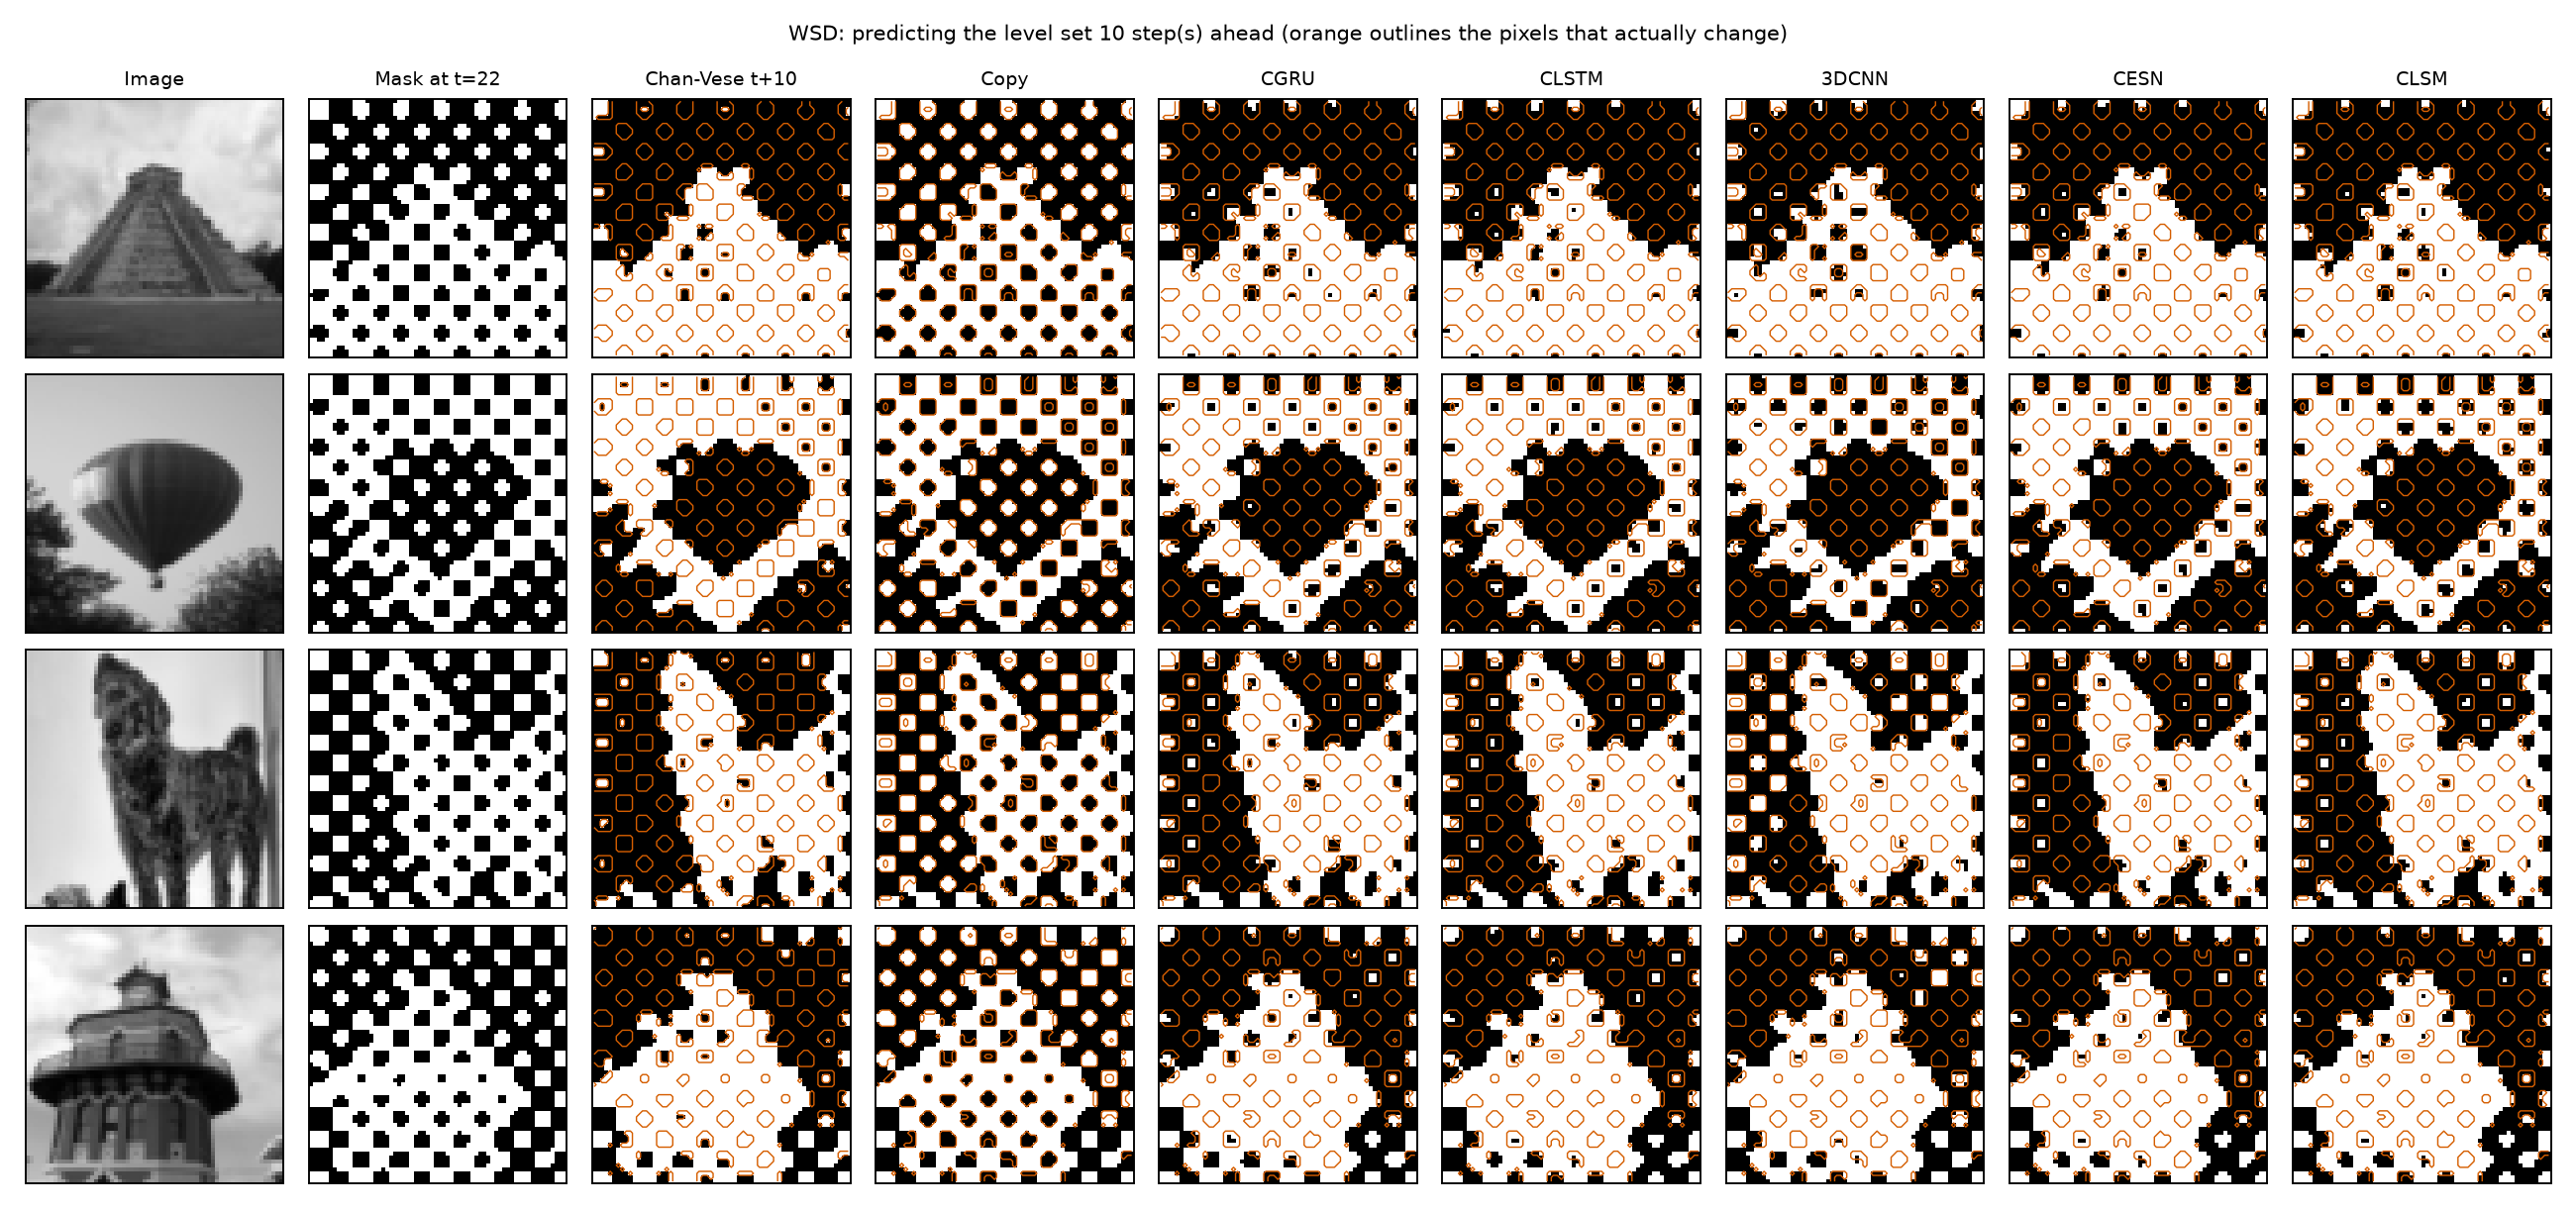
\includegraphics[width=\textwidth]{qualitative_wsd_G.png}
\caption{Predictions ten iterations ahead, at the moment of each sequence where
the front moves most. Orange outlines the pixels whose label changes, which is
the region change IoU scores; everything outside it is reproduced by copying.}
\label{fig:qualitative}
\end{figure}

\begin{figure}[t]
\centering
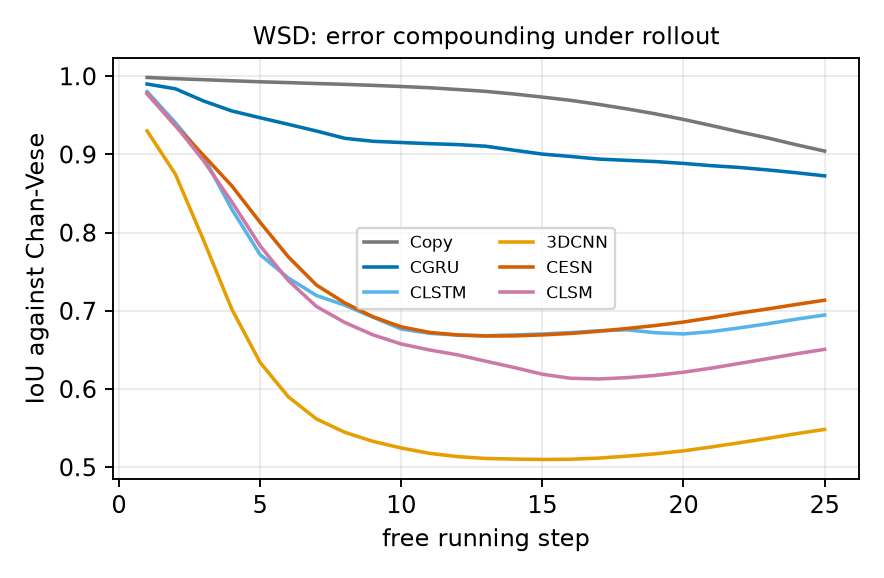
\includegraphics[width=0.49\textwidth]{rollout_wsd_G.png}
\hfill
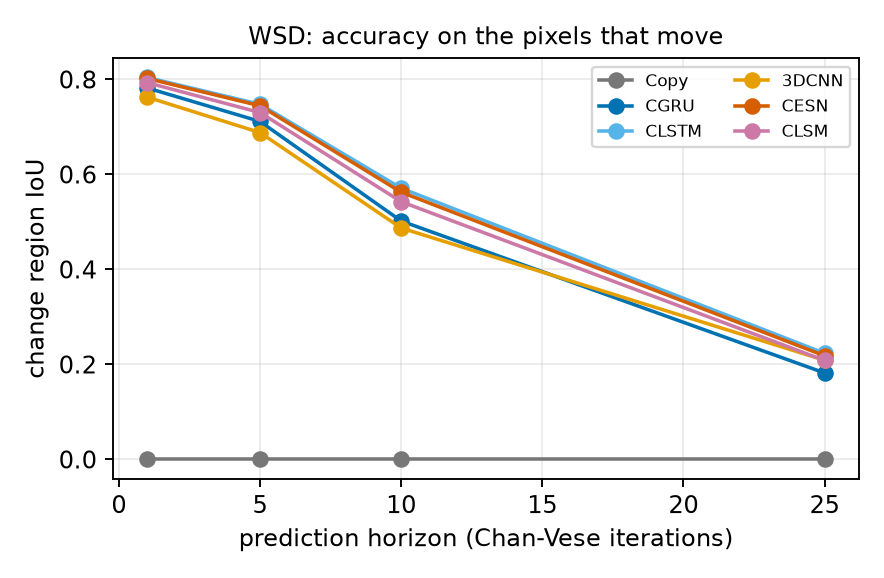
\includegraphics[width=0.49\textwidth]{horizons_wsd_G.png}
\caption{Left: free running rollout, where errors compound and the copy
control's advantage decays. Right: change region accuracy against prediction
horizon. The horizon the original used is the leftmost point, where the task is
nearly solved by the identity.}
\label{fig:curves}
\end{figure}

\begin{figure}[t]
\centering
\includegraphics[width=0.62\textwidth]{sweep_esn.png}
\caption{The reservoir parameters the original blamed for the echo state
network's failure, swept directly under a configuration in which the model
trains. One seed per cell: the variation shown is comparable to the seed to
seed spread of a fixed configuration, so this is a map of noise as much as of
structure, and is reported as inconclusive rather than as a tuning law.}
\label{fig:sweep}
\end{figure}

\begin{table}[t]
\centering\small
\begin{tabular}{lrrrrrr}
\toprule
model & IoU & change IoU & rollout IoU & rollout change IoU & boundary F1 & fit (s) \\
\midrule
Copy previous \emph{(control)} & 0.993 {\scriptsize$\pm$ 0.000} & 0.000 {\scriptsize$\pm$ 0.000} & 0.966 {\scriptsize$\pm$ 0.000} & 0.000 {\scriptsize$\pm$ 0.000} & 0.998 {\scriptsize$\pm$ 0.000} & 0 \\
White noise \emph{(control)} & 0.335 {\scriptsize$\pm$ 0.000} & 0.335 {\scriptsize$\pm$ 0.000} & 0.335 {\scriptsize$\pm$ 0.000} & 0.355 {\scriptsize$\pm$ 0.001} & 0.765 {\scriptsize$\pm$ 0.000} & 0 \\
CGRU & 0.420 {\scriptsize$\pm$ 0.002} & 0.126 {\scriptsize$\pm$ 0.007} & 0.504 {\scriptsize$\pm$ 0.004} & 0.239 {\scriptsize$\pm$ 0.007} & 0.762 {\scriptsize$\pm$ 0.001} & 8 \\
CLSTM & 0.420 {\scriptsize$\pm$ 0.002} & 0.126 {\scriptsize$\pm$ 0.007} & 0.504 {\scriptsize$\pm$ 0.004} & 0.239 {\scriptsize$\pm$ 0.007} & 0.762 {\scriptsize$\pm$ 0.001} & 8 \\
CRNN & 0.420 {\scriptsize$\pm$ 0.002} & 0.126 {\scriptsize$\pm$ 0.007} & 0.504 {\scriptsize$\pm$ 0.004} & 0.239 {\scriptsize$\pm$ 0.007} & 0.762 {\scriptsize$\pm$ 0.001} & 8 \\
3DCNN & 0.420 {\scriptsize$\pm$ 0.002} & 0.126 {\scriptsize$\pm$ 0.007} & 0.504 {\scriptsize$\pm$ 0.004} & 0.239 {\scriptsize$\pm$ 0.007} & 0.762 {\scriptsize$\pm$ 0.001} & 5 \\
CESN \emph{(reservoir)} & 0.420 {\scriptsize$\pm$ 0.002} & 0.126 {\scriptsize$\pm$ 0.007} & 0.504 {\scriptsize$\pm$ 0.004} & 0.239 {\scriptsize$\pm$ 0.007} & 0.762 {\scriptsize$\pm$ 0.001} & 8 \\
\bottomrule
\end{tabular}
\caption{WSD. The published configuration reproduced: fully connected head, window one, one step ahead, SGD at learning rate 0.1 with weight decay 0.1. Every model collapses to a constant output, and none approaches the copy control.}
\label{tab:blockA}
\end{table}

\begin{table}[t]
\centering\small
\begin{tabular}{lrrrrrr}
\toprule
model & IoU & change IoU & rollout IoU & rollout change IoU & boundary F1 & fit (s) \\
\midrule
Copy previous \emph{(control)} & 0.993 {\scriptsize$\pm$ 0.000} & 0.000 {\scriptsize$\pm$ 0.000} & 0.971 {\scriptsize$\pm$ 0.000} & 0.000 {\scriptsize$\pm$ 0.000} & 0.998 {\scriptsize$\pm$ 0.000} & 0 \\
White noise \emph{(control)} & 0.336 {\scriptsize$\pm$ 0.000} & 0.338 {\scriptsize$\pm$ 0.000} & 0.336 {\scriptsize$\pm$ 0.000} & 0.336 {\scriptsize$\pm$ 0.001} & 0.759 {\scriptsize$\pm$ 0.000} & 0 \\
CGRU & 0.457 {\scriptsize$\pm$ 0.002} & 0.170 {\scriptsize$\pm$ 0.004} & 0.548 {\scriptsize$\pm$ 0.004} & 0.278 {\scriptsize$\pm$ 0.007} & 0.759 {\scriptsize$\pm$ 0.001} & 23 \\
CLSTM & 0.457 {\scriptsize$\pm$ 0.002} & 0.170 {\scriptsize$\pm$ 0.004} & 0.548 {\scriptsize$\pm$ 0.004} & 0.278 {\scriptsize$\pm$ 0.007} & 0.759 {\scriptsize$\pm$ 0.001} & 21 \\
CRNN & 0.457 {\scriptsize$\pm$ 0.002} & 0.170 {\scriptsize$\pm$ 0.004} & 0.548 {\scriptsize$\pm$ 0.004} & 0.278 {\scriptsize$\pm$ 0.007} & 0.759 {\scriptsize$\pm$ 0.001} & 21 \\
3DCNN & 0.457 {\scriptsize$\pm$ 0.002} & 0.170 {\scriptsize$\pm$ 0.004} & 0.548 {\scriptsize$\pm$ 0.004} & 0.278 {\scriptsize$\pm$ 0.007} & 0.759 {\scriptsize$\pm$ 0.001} & 23 \\
CESN \emph{(reservoir)} & 0.457 {\scriptsize$\pm$ 0.002} & 0.170 {\scriptsize$\pm$ 0.004} & 0.548 {\scriptsize$\pm$ 0.004} & 0.278 {\scriptsize$\pm$ 0.007} & 0.759 {\scriptsize$\pm$ 0.001} & 21 \\
\bottomrule
\end{tabular}
\caption{BSD. The published configuration reproduced: fully connected head, window one, one step ahead, SGD at learning rate 0.1 with weight decay 0.1. Every model collapses to a constant output, and none approaches the copy control.}
\label{tab:blockAbsd}
\end{table}

\begin{table}[t]
\centering\small
\begin{tabular}{lrrrrrr}
\toprule
model & IoU & change IoU & rollout IoU & rollout change IoU & boundary F1 & fit (s) \\
\midrule
CGRU & 0.806 {\scriptsize$\pm$ 0.001} & 0.332 {\scriptsize$\pm$ 0.006} & 0.846 {\scriptsize$\pm$ 0.004} & 0.349 {\scriptsize$\pm$ 0.005} & 0.909 {\scriptsize$\pm$ 0.001} & 15 \\
CLSTM & 0.801 {\scriptsize$\pm$ 0.001} & 0.324 {\scriptsize$\pm$ 0.010} & 0.839 {\scriptsize$\pm$ 0.005} & 0.345 {\scriptsize$\pm$ 0.013} & 0.906 {\scriptsize$\pm$ 0.001} & 15 \\
3DCNN & 0.796 {\scriptsize$\pm$ 0.001} & 0.286 {\scriptsize$\pm$ 0.005} & 0.843 {\scriptsize$\pm$ 0.002} & 0.332 {\scriptsize$\pm$ 0.009} & 0.907 {\scriptsize$\pm$ 0.000} & 10 \\
CESN \emph{(reservoir)} & 0.786 {\scriptsize$\pm$ 0.000} & 0.302 {\scriptsize$\pm$ 0.003} & 0.833 {\scriptsize$\pm$ 0.005} & 0.314 {\scriptsize$\pm$ 0.009} & 0.899 {\scriptsize$\pm$ 0.001} & 15 \\
CLSM \emph{(spiking reservoir)} & 0.587 {\scriptsize$\pm$ 0.040} & 0.383 {\scriptsize$\pm$ 0.044} & 0.372 {\scriptsize$\pm$ 0.029} & 0.395 {\scriptsize$\pm$ 0.075} & 0.810 {\scriptsize$\pm$ 0.031} & 8 \\
\bottomrule
\end{tabular}
\caption{WSD. The same head and task with AdamW instead. The recipe, not the head alone, explains the collapse in Table~\ref{tab:blockA}.}
\label{tab:blockF}
\end{table}

\begin{table}[t]
\centering\small
\begin{tabular}{lrrrrrr}
\toprule
model & IoU & change IoU & rollout IoU & rollout change IoU & boundary F1 & fit (s) \\
\midrule
CGRU & 0.834 {\scriptsize$\pm$ 0.000} & 0.321 {\scriptsize$\pm$ 0.008} & 0.867 {\scriptsize$\pm$ 0.002} & 0.366 {\scriptsize$\pm$ 0.007} & 0.931 {\scriptsize$\pm$ 0.001} & 35 \\
CLSTM & 0.830 {\scriptsize$\pm$ 0.002} & 0.310 {\scriptsize$\pm$ 0.003} & 0.863 {\scriptsize$\pm$ 0.002} & 0.358 {\scriptsize$\pm$ 0.010} & 0.928 {\scriptsize$\pm$ 0.002} & 37 \\
3DCNN & 0.820 {\scriptsize$\pm$ 0.000} & 0.309 {\scriptsize$\pm$ 0.005} & 0.850 {\scriptsize$\pm$ 0.001} & 0.340 {\scriptsize$\pm$ 0.004} & 0.918 {\scriptsize$\pm$ 0.000} & 26 \\
CESN \emph{(reservoir)} & 0.818 {\scriptsize$\pm$ 0.002} & 0.316 {\scriptsize$\pm$ 0.013} & 0.847 {\scriptsize$\pm$ 0.005} & 0.351 {\scriptsize$\pm$ 0.013} & 0.915 {\scriptsize$\pm$ 0.002} & 35 \\
CLSM \emph{(spiking reservoir)} & 0.622 {\scriptsize$\pm$ 0.026} & 0.426 {\scriptsize$\pm$ 0.053} & 0.396 {\scriptsize$\pm$ 0.031} & 0.425 {\scriptsize$\pm$ 0.065} & 0.796 {\scriptsize$\pm$ 0.038} & 29 \\
\bottomrule
\end{tabular}
\caption{BSD. The same head and task with AdamW instead. The recipe, not the head alone, explains the collapse in Table~\ref{tab:blockA}.}
\label{tab:blockFbsd}
\end{table}

\begin{table}[t]
\centering\small
\begin{tabular}{lrrrrrr}
\toprule
model & IoU & change IoU & rollout IoU & rollout change IoU & boundary F1 & fit (s) \\
\midrule
Copy previous \emph{(control)} & 0.925 {\scriptsize$\pm$ 0.000} & 0.000 {\scriptsize$\pm$ 0.000} & 0.967 {\scriptsize$\pm$ 0.000} & 0.000 {\scriptsize$\pm$ 0.000} & 0.956 {\scriptsize$\pm$ 0.000} & 0 \\
White noise \emph{(control)} & 0.336 {\scriptsize$\pm$ 0.000} & 0.336 {\scriptsize$\pm$ 0.001} & 0.335 {\scriptsize$\pm$ 0.000} & 0.337 {\scriptsize$\pm$ 0.002} & 0.732 {\scriptsize$\pm$ 0.000} & 0 \\
CGRU & 0.964 {\scriptsize$\pm$ 0.000} & 0.523 {\scriptsize$\pm$ 0.018} & 0.804 {\scriptsize$\pm$ 0.085} & 0.520 {\scriptsize$\pm$ 0.187} & 0.993 {\scriptsize$\pm$ 0.000} & 53 \\
CLSTM & 0.963 {\scriptsize$\pm$ 0.001} & 0.531 {\scriptsize$\pm$ 0.043} & 0.784 {\scriptsize$\pm$ 0.085} & 0.532 {\scriptsize$\pm$ 0.199} & 0.993 {\scriptsize$\pm$ 0.001} & 41 \\
CRNN & 0.963 {\scriptsize$\pm$ 0.002} & 0.549 {\scriptsize$\pm$ 0.014} & 0.720 {\scriptsize$\pm$ 0.044} & 0.672 {\scriptsize$\pm$ 0.049} & 0.993 {\scriptsize$\pm$ 0.001} & 33 \\
3DCNN & 0.938 {\scriptsize$\pm$ 0.001} & 0.490 {\scriptsize$\pm$ 0.005} & 0.579 {\scriptsize$\pm$ 0.003} & 0.731 {\scriptsize$\pm$ 0.004} & 0.992 {\scriptsize$\pm$ 0.000} & 47 \\
CESN \emph{(reservoir)} & 0.962 {\scriptsize$\pm$ 0.002} & 0.515 {\scriptsize$\pm$ 0.044} & 0.806 {\scriptsize$\pm$ 0.087} & 0.543 {\scriptsize$\pm$ 0.179} & 0.993 {\scriptsize$\pm$ 0.001} & 40 \\
CLSM \emph{(spiking reservoir)} & 0.962 {\scriptsize$\pm$ 0.002} & 0.511 {\scriptsize$\pm$ 0.028} & 0.733 {\scriptsize$\pm$ 0.053} & 0.668 {\scriptsize$\pm$ 0.055} & 0.993 {\scriptsize$\pm$ 0.001} & 50 \\
CESN \emph{(reservoir)}, ridge readout & 0.646 {\scriptsize$\pm$ 0.030} & 0.305 {\scriptsize$\pm$ 0.015} & 0.401 {\scriptsize$\pm$ 0.030} & 0.375 {\scriptsize$\pm$ 0.048} & 0.826 {\scriptsize$\pm$ 0.016} & 1 \\
CLSM \emph{(spiking reservoir)}, ridge readout & 0.437 {\scriptsize$\pm$ 0.013} & 0.235 {\scriptsize$\pm$ 0.008} & 0.394 {\scriptsize$\pm$ 0.007} & 0.327 {\scriptsize$\pm$ 0.021} & 0.713 {\scriptsize$\pm$ 0.007} & 3 \\
\bottomrule
\end{tabular}
\caption{WSD. The corrected setting: spatial decoder head, window four, ten iterations ahead, AdamW. Change IoU scores only the pixels whose label differs between the last input mask and the target.}
\label{tab:blockG}
\end{table}

\begin{table}[t]
\centering\small
\begin{tabular}{lrrrrrr}
\toprule
model & IoU & change IoU & rollout IoU & rollout change IoU & boundary F1 & fit (s) \\
\midrule
Copy previous \emph{(control)} & 0.922 {\scriptsize$\pm$ 0.000} & 0.000 {\scriptsize$\pm$ 0.000} & 0.970 {\scriptsize$\pm$ 0.000} & 0.000 {\scriptsize$\pm$ 0.000} & 0.956 {\scriptsize$\pm$ 0.000} & 0 \\
White noise \emph{(control)} & 0.336 {\scriptsize$\pm$ 0.000} & 0.337 {\scriptsize$\pm$ 0.000} & 0.336 {\scriptsize$\pm$ 0.000} & 0.320 {\scriptsize$\pm$ 0.002} & 0.724 {\scriptsize$\pm$ 0.000} & 0 \\
CGRU & 0.971 {\scriptsize$\pm$ 0.000} & 0.593 {\scriptsize$\pm$ 0.008} & 0.766 {\scriptsize$\pm$ 0.021} & 0.544 {\scriptsize$\pm$ 0.009} & 0.996 {\scriptsize$\pm$ 0.000} & 104 \\
CLSTM & 0.970 {\scriptsize$\pm$ 0.001} & 0.581 {\scriptsize$\pm$ 0.016} & 0.815 {\scriptsize$\pm$ 0.041} & 0.408 {\scriptsize$\pm$ 0.096} & 0.995 {\scriptsize$\pm$ 0.000} & 104 \\
CRNN & 0.970 {\scriptsize$\pm$ 0.000} & 0.578 {\scriptsize$\pm$ 0.010} & 0.812 {\scriptsize$\pm$ 0.044} & 0.474 {\scriptsize$\pm$ 0.077} & 0.996 {\scriptsize$\pm$ 0.000} & 106 \\
3DCNN & 0.958 {\scriptsize$\pm$ 0.000} & 0.505 {\scriptsize$\pm$ 0.003} & 0.608 {\scriptsize$\pm$ 0.009} & 0.698 {\scriptsize$\pm$ 0.010} & 0.994 {\scriptsize$\pm$ 0.000} & 84 \\
CESN \emph{(reservoir)} & 0.968 {\scriptsize$\pm$ 0.001} & 0.553 {\scriptsize$\pm$ 0.005} & 0.786 {\scriptsize$\pm$ 0.055} & 0.519 {\scriptsize$\pm$ 0.036} & 0.995 {\scriptsize$\pm$ 0.000} & 100 \\
CLSM \emph{(spiking reservoir)} & 0.968 {\scriptsize$\pm$ 0.001} & 0.552 {\scriptsize$\pm$ 0.012} & 0.758 {\scriptsize$\pm$ 0.007} & 0.572 {\scriptsize$\pm$ 0.023} & 0.995 {\scriptsize$\pm$ 0.000} & 138 \\
CESN \emph{(reservoir)}, ridge readout & 0.650 {\scriptsize$\pm$ 0.026} & 0.320 {\scriptsize$\pm$ 0.031} & 0.398 {\scriptsize$\pm$ 0.038} & 0.377 {\scriptsize$\pm$ 0.095} & 0.825 {\scriptsize$\pm$ 0.017} & 3 \\
CLSM \emph{(spiking reservoir)}, ridge readout & 0.470 {\scriptsize$\pm$ 0.010} & 0.282 {\scriptsize$\pm$ 0.008} & 0.437 {\scriptsize$\pm$ 0.012} & 0.325 {\scriptsize$\pm$ 0.017} & 0.694 {\scriptsize$\pm$ 0.007} & 7 \\
\bottomrule
\end{tabular}
\caption{BSD. The corrected setting: spatial decoder head, window four, ten iterations ahead, AdamW. Change IoU scores only the pixels whose label differs between the last input mask and the target.}
\label{tab:blockGbsd}
\end{table}



\section{Results}

\subsection{The published configuration reproduces nothing that can be compared}

Under the original's own recipe (Table~\ref{tab:blockA}) every architecture
returns the same numbers to three decimal places: \Awsdgruiou{} IoU on WSD for
the gated recurrent unit, the long short term memory, the plain recurrent
network, the 3D convolutional network and the echo state network alike. The
cause is visible in the predictions rather than the metrics: the models emit a
constant 0.5 everywhere, so thresholding produces one fixed mask for every
input. Weight decay of 0.1 applied at a learning rate of 0.1 shrinks the
encoder faster than the loss can shape it.

Two consequences follow. First, the differences between cells reported in the
original are differences between degenerate models. Second, the white noise
control (\Awsdnoiseiou{} IoU) is not a floor that a collapsed model clears by
learning; it is simply what a fixed mask scores against a slowly moving target.

The copy control settles the point. Predicting that nothing changes scores
\Awsdcopyiou{} IoU on WSD and \Absdcopyiou{} on BSD, above every figure in the
original study. Whatever those models were ranked on, it was not the ability to
predict the level set.

\subsection{The optimiser and the head are separable causes}

Replacing the optimiser alone (Table~\ref{tab:blockF}) removes the collapse:
the same fully connected head now reaches \Fwsdgruiou{} IoU for the gated
recurrent unit and \Fwsdesniou{} for the echo state network, with change IoU of
\Fwsdgruchangeiou{} and \Fwsdesnchangeiou{} respectively. The architecture was
never the reason nothing trained.

Replacing the head as well (Table~\ref{tab:blockG}) lifts every model to about
\Gwsdgruiou{} IoU. The gap between the two heads is far larger than any gap
between recurrent cells, which is the central measurement of this paper: the
original compared cells through a bottleneck that dominated the result.

\subsection{Once the task discriminates, the cells do not}

At a ten iteration horizon with a four frame window, scoring only the pixels
that move, the ordering the original reported does not appear at all
(Table~\ref{tab:blockG}). On WSD the change IoU values are
\Gwsdgruchangeiou{} (CGRU), \Gwsdlstmchangeiou{} (CLSTM),
\Gwsdrnnchangeiou{} (CRNN), \Gwsdesnchangeiou{} (CESN) and
\Gwsdlsmchangeiou{} (CLSM), a spread comparable to the seed to seed standard
deviation of each arm. On BSD the same holds. An untrained random reservoir,
analogue or spiking, matches networks trained end to end.

The original reported the echo state network at roughly a third of the gated
recurrent unit's IoU. That gap is not reproduced here under any configuration
in which both models train at all.

\subsection{What the cheap readout costs}

Fitting only a linear readout in closed form, with no backpropagation anywhere
and a frozen random encoder, takes \Gwsdesnridgefitseconds{} seconds on WSD
against \Gwsdesnfitseconds{} seconds for the gradient trained reservoir, a
reduction of more than an order of magnitude. It is also clearly worse:
\Gwsdesnridgechangeiou{} change IoU against \Gwsdesnchangeiou{}. The spiking
liquid loses more than the analogue reservoir does
(\Gwsdlsmridgechangeiou{}), which is consistent with its state being a
filtered spike train rather than a continuous activation.

This is the honest form of the reservoir argument. A reservoir is cheap when it
is fitted the way reservoirs are meant to be fitted, and on this task that
cheapness costs accuracy. Training the readout by gradient descent, as the
original did, buys the accuracy back and gives up the cost advantage: its
fitting time is then the same as a trained recurrent network's.

\subsection{Rollout separates conservative models from dynamic ones}

Under free running rollout the global and change metrics move in opposite
directions. The gated models keep a higher whole image IoU
(\Gwsdgrurolloutiou{} for CGRU) while the 3D convolutional network and the
reservoirs score higher on the moving front (\GwsdTdcnnrolloutchangeiou{}
and \Gwsdesnrolloutchangeiou{} against \Gwsdgrurolloutchangeiou{}). A model
that predicts little change tracks a slow target well in aggregate and captures
none of its motion. Reporting only one of these numbers would support either
conclusion, which is why both are in the table.

\subsection{The parameters the original blamed do not move the result}

Sweeping the spectral radius from 0.5 to 1.5 and the leaking rate from 0.0078
to 1.0, in a configuration where the model trains, moves change IoU between
\esnsweepmin{} and \esnsweepmax{} across \esnsweepcells{} cells, a standard
deviation of \esnsweepsd{} (Figure~\ref{fig:sweep}). For comparison, three
seeds of one fixed configuration vary by \seedrepsd{}. The reservoir
parameters the original identified as the cause of failure change the outcome
less than the random seed does.

The liquid's parameters behave the same way. Its firing rate responds strongly
to the threshold, from \lsmfiringmin{} to \lsmfiringmax{} spikes per neuron per
step, while its accuracy stays between \lsmsweepmin{} and \lsmsweepmax{}. The
liquid is therefore robust in accuracy and adjustable in cost, which is the
useful direction for a spiking model.

\subsection{Training on the part of the sequence that moves}

The level set is static for tens of iterations and then collapses, so uniform
sampling spends most of training on frames where nothing happens. Restricting
training to samples whose target differs from the input by at least half a
percent of pixels (Table~\ref{tab:blockH}) leaves the comparison unchanged
(CGRU \Hwsdgruchangeiou{}, CESN \Hwsdesnchangeiou{}, CLSM
\Hwsdlsmchangeiou{}) while reducing the training set. The stillness was
neither helping nor hurting; it was simply padding.


\section{Discussion}

\subsection{What the original measured}

The dissertation's conclusion was that echo state networks cannot learn the
variational level set, and that the leaking rate and spectral radius are
responsible. The first half is not supported by the experiments reported here:
under every configuration in which the models train at all, the echo state
network is within seed noise of the trained recurrent networks. The second half
is a claim about a parameter sensitivity that this study cannot confirm either
(Table~\ref{tab:blockA} and the sweep): the response surface over spectral
radius and leak is not systematic at the resolution a single seed per cell can
resolve, and the differences it shows are smaller than the seed to seed spread
of a fixed configuration.

What the original did measure, we think, is three properties of its own setup:
an optimiser that prevents training, a readout that destroys the geometry the
task is about, and a horizon at which the identity function is close to
optimal. None of these is a property of reservoir computing.

\subsection{Why the head matters so much here}

The target mask differs from the input mask in a small band around the moving
front. A decoder with a skip connection can express "copy, then edit the band";
a globally pooled vector cannot, because every pixel of the output must be
reconstructed from a representation that has already discarded position. This
is why the head changes results by more than the choice of recurrent cell does,
and why a study comparing cells has to control for it.

\subsection{What the reservoirs are actually worth}

On accuracy, nothing separates them from trained networks on this task. On
cost, the picture depends entirely on how the readout is fitted. Trained by
gradient descent, as the original did, a reservoir costs what a gated network
costs and is therefore pointless. Fitted in closed form, it is more than an
order of magnitude cheaper and gives up a substantial amount of accuracy.

The spiking liquid adds a further consideration the analogue reservoir does
not: its state is a filtered spike train with a measured firing rate of about a
quarter, which is the quantity that would matter on neuromorphic hardware where
cost is counted in spikes rather than in multiplications. On this task it
matches the analogue reservoir when its readout is trained and falls behind it
when the readout is solved.

\subsection{A methodological point that outlives this task}

A slowly evolving partial differential equation is an adversarial case for
whole image overlap metrics. Any metric dominated by the static part of the
signal will rank a model that predicts stasis above a model that predicts
motion imperfectly, and both above nothing. Three cheap habits avoid this:
report the identity baseline, restrict the metric to the region that changes,
and evaluate at a horizon long enough that the identity baseline fails. The
first alone would have caught the problem in the original study.


\section{Limitations}

A single consumer GPU, $64 \times 64$ inputs, and two of the original's four
databases. The CIFAR scale experiments of the original (millions of generated
examples) are not reproduced. One PDE, one solver, one parameter setting of
that solver. The spatial head's skip connection includes the previous mask
explicitly, which is the right inductive bias for this task and would not
transfer unchanged to a task whose output is unrelated to its input.

\section{Reproducing this}

Code, configurations and the exact commands are at
\url{https://github.com/LeparaLaMapara/esn-levelset-study}. Every number in
this paper is generated from the run directories by
\texttt{scripts/make\_paper\_numbers.py}; none is typed into the text.

\end{document}
